% latex packages to load.
\documentclass[12pt]{article}
\usepackage{geometry}
\geometry{a4paper}
%\geometry{landscape}
\usepackage[parfill]{parskip}    % Activate to begin paragraphs with an empty line rather than an indent
\usepackage{graphicx}
\usepackage{amssymb}
\usepackage{epstopdf}
\usepackage{courier}
\usepackage{fancyhdr}
\usepackage{fullpage}
\usepackage{appendix}
\usepackage{newclude}
\usepackage{datetime}
\usepackage{hyperref}
\usepackage{color}
\usepackage{multicol}
\usepackage{tabularx}
\usepackage{enumerate}
\usepackage{enumitem}
\usepackage{listings}
\usepackage{wallpaper}
\usepackage{lastpage}
\usepackage{titling}
\usepackage{multind}
\usepackage[table]{xcolor}
\usepackage{mathtools}

\usepackage{tikz}
\usetikzlibrary{shapes,arrows}

\tikzstyle{block} = [rectangle, draw, text width = 6em, text centered, rounded corners, minimum height = 4em]
\tikzstyle{inputblock} = [rectangle, draw, text width = 24em, minimum height = 2.5em]
\tikzstyle{autographblock} = [rectangle, draw, fill = black!1, text height = 0, text depth = 2cm,text width = 24em, minimum height = 8em]
\tikzstyle{cloud} = [ellipse, draw, minimum height = 4em]
\tikzstyle{line} = [draw, -latex']

% INDEXES
\makeindex{modules}
\newcommand{\usemodule}[1]{\index{modules}{#1}\texttt{#1}}

\definecolor{gray}{rgb}{0.5,0.5,0.5}
\definecolor{tableheader}{rgb}{0.7,0.7,0.7}

\setlist[description]{style=nextline}
\renewcommand{\familydefault}{\sfdefault}

% link setup
\hypersetup{
    colorlinks,
    citecolor=black,
    filecolor=black,
    linkcolor=black,
    urlcolor=black,
}

\DeclareGraphicsRule{.tif}{png}{.png}{`convert #1 `dirname #1`/`basename #1 .tif`.png}

% usefull commands:
\newcommand{\seeref}[1]{\ref{#1} p.\pageref{#1}}
\newcommand{\seeone}[1]{ (zie \ref{#1} p.\pageref{#1})}
\newcommand{\seesee}[2]{ (zie \ref{#1} p.\pageref{#1},  \ref{#2} p.\pageref{#2})}

% style for code blocks
\lstset{
    linewidth=1\textwidth,
    breaklines=true,
    numbers=left,                   % where to put the line-numbers
    numberstyle=\tiny\color{gray},  % the style that is used for the line-numbers
    stepnumber=1,                   % the step between two line-numbers. If it's 1, each line 
    numbersep=5pt, 
    basicstyle=\ttfamily\footnotesize,
}

% Header and Footer settings
%\URCornerWallPaper{0.13}{img/dop/koptekstlogo.png}
\pagestyle{fancy}
\fancyhead{}
\renewcommand{\headrulewidth}{0pt}


\fancyfoot[L]{Technisch ontwerp - \customer}
\fancyfoot[C]{}
\fancyfoot[R]{\textbf{\thepage}\ / \pageref{LastPage}}

% Settings for table of contents.	
\setcounter{secnumdepth}{4}
\setcounter{tocdepth}{3}


\makeatletter
% some extra spacing for the table of contents
\renewcommand{\l@subsection}{\@dottedtocline{2}{1.5em}{3em}}
\renewcommand{\l@subsubsection}{\@dottedtocline{2}{2.7em}{4em}}

\renewcommand\paragraph{%
   \@startsection{paragraph}{4}{0mm}%
      {-\baselineskip}%
      {.5\baselineskip}%
      {\normalfont\normalsize\bfseries}}
\makeatother

% Define variables	
\newcommand{\customer}{Dimpact}
\newcommand{\projectname}{Dimpact Drupal distributie}
\newcommand{\thecustomer}{\customer }
\newcommand{\customerdomain}{gemeente.nl}
\newcommand{\customerdomainfull}{http://www.gemeente.nl}
\newcommand{\customerdomainuc}{Gemeente.nl}
\newcommand{\authors}{ Bas van der Heijden \\ & Patrick Kraaij \\ & Maurits Lawende }


% Voorblad of the documentq
\ThisLRCornerWallPaper{0.8}{img/dop/voorbladlogo.png}

\title{\textbf{\projectname} \\ Technisch Ontwerp}
\pretitle{\begin{flushleft}\LARGE}
\posttitle{\par\end{flushleft}}

\author{}  % skippen we voor maketitle
\date{}

% The actual Document:
\begin{document}
 \maketitle
 \vspace{-2.6cm}
  \begin{flushright}
      \ThisLRCornerWallPaper{0.8}{img/dop/voorbladlogo.png}

  \maketitle
 \vspace{-2.6cm}
  \begin{flushright}
\begin{tabularx}{4.6cm}{ X }
Dutch Open Projects         \\
Doornseweg 12                   \\  
3832 RL Leusden                 \\
T: +31[0]33 - 4 50 50 50        \\
F: +31[0]33 - 4 50 50 57        
\\*
\\*
\\*
\\*
\\*
\\*
\\*
\\*
\\*
\\*
\\*
\\*
\\*
\\*
\\*
\\*
\\*
\\*
\\*
\\*



\footnotesize
\copyright All rights reserved.         \\*
\footnotesize
No part of the contents of this publication may be reproduced, stored in a data processing system or transmitted in any form or by any means without the written permission of Dutch Open Projects B.V.

\end{tabularx}
\end{flushright}

\begin{tabularx}{\linewidth}{ p{3cm} X }
  Plaats & Leusden                                \\
  Laatst bijgewerkt & \ddmmyyyydate \today        \\
  Auteurs & \authors                          \\
  Versie & \version                                    \\
\end{tabularx}
\pagebreak



  \end{flushright}
  
 \null
 \vfill    
  \begin{tabularx}{\linewidth}{ p{3cm} X }
    Plaats & Leusden                                                           \\
    Laatst bijgewerkt & \ddmmyyyydate \today           \\
    Auteurs & \authors                                                 \\
    Versie & 0.1                                                                       \\
  \end{tabularx}
\pagebreak

%\section{Beheer}

\begin{tabularx}{\linewidth}{| p{2.5cm} | p{2.5cm} | X | p{2.5cm} |}
\rowcolor{tableheader}
\hline
\textbf{Versie} & \textbf{Datum} & \textbf{Omschrijving} &  \textbf{Auteur}			\\ \hline
0.1 & 17-12-2012 & Draft 											& DOP			\\ \hline
0.2 & 20-12-2012 & Inventarisatie deeloplevering 						& DOP			\\ \hline
0.3 & 08-01-2013 & Toevoeging: cookies, sms, rollen rechten, todo's					& DOP			\\ \hline
0.9 & 09-01-2013 & Toevoeging: HR, gebruikersrollen, persmissieoverzicht & DOP \\ \hline
1.0 & 14-03-2013 & Feedback H. Morang verwerkt & DOP \\ \hline
1.1 & 25-03-2013 & Feedback H. Morang, B. Ot, M. Welleman, J. Zigerman & DOP\\ \hline
1.2 & 29-04-2013 & Feedback H. Morang (punt 1,3,4) & DOP\\ \hline
%versie & datum & omschrijving & auteur             	\\ \hline
\end{tabularx}

\subsection{Akkoord}
Voor akkoord:\\ \\
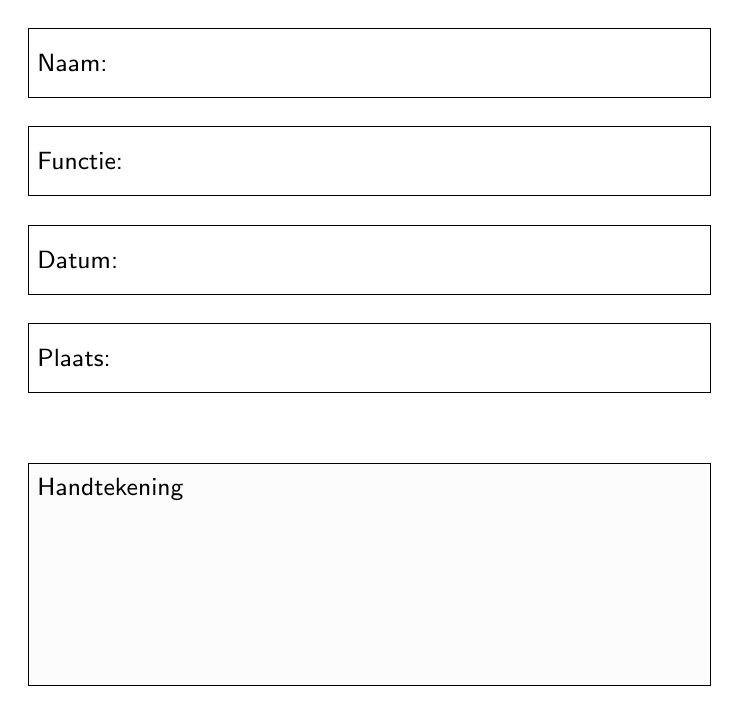
\begin{tikzpicture}
\tikzstyle{every node}=[font=\small];
\node [inputblock] (names) {Naam:};
\node [inputblock, below of = names, node distance = 1.25cm] (function) {Functie:};
\node [inputblock, below of = function, node distance = 1.25cm] (dates) {Datum:};
\node [inputblock, below of = dates, node distance = 1.25cm] (place) {Plaats:};
\node [autographblock, below of = place, node distance = 2.75cm] (autograph) {Handtekening};
\end{tikzpicture}



% table of contents
\renewcommand*\contentsname{Inhoudsopgave}
\tableofcontents

\pagebreak


% The document

% Introductie

\section{Introductie}

\subsection{Management summary}
In dit document wordt de technische implementatie beschreven. Het is een blauwdruk voor ontwikkelaars. 

\subsection{Opbouw document}
Dit document dient als leidraad voor de bouw van dit project. Het belangrijkste onderdeel ervan zijn daarom de componenten. Deze zijn uitgesplitst naar componenten voor internet\seeone{internet} en intranet\seeone{intranet}.  Componenten bieden een opsplitsing van de functionaliteiten binnen de website, zowel zichtbaar als niet zichtbaar. Tijdens de bouw zal een ontwikkelaar aan \'{e}\'{e}n specifiek component tegelijk werken. Daarnaast worden in dit document een aantal randzaken zoals deployment\seeone{deployment} en performance\seeone{performance} en algemene eisen\seeone{algemeen} beschreven in eerdere hoofdstukken. In de appendix vindt met een overzicht van Drupal specifieke zaken zoals content types en views.
\section{Basiselementen, terminologie en definities}

Elk softwaresysteem hanteert bepaald taalgebruik en termen. Dit om een eenduidige betekenis van een term te defini\"eren. Voor het schrijf- en leesgemak van de ontwikkelaars worden dan ook de termen gebruikt die bij Drupal gangbaar zijn. Echter voor een niet-ontwikkelaar of een niet-Drupal gebruiker kan dit verwarring opleveren. 

\begin{description}

\item[Drupal] Drupal is het gekozen Content Management Systeem wat als framework dient voor de bouw van de nieuwe website. Drupal is Open Source CMS welke geschreven is in PHP. 

\item[Modules] Drupal is een modulair gebaseerd systeem. Een module is een verzameling van code welke als uitbreiding dient. In andere systemen wordt dit ook wel een plug-in of extensie genoemd. 

\item[Contrib (contributed) modules] Wanneer gesproken wordt over contrib of contributed modules, wordt hiermee bedoeld de modules die beschikbaar zijn op drupal.org. Dit zijn modules die beschikbaar zijn gesteld door communityleden, welke vrij te verkrijgen zijn. 

\item[Custom modules] Hiermee wordt bedoeld modules die op maat zijn gemaakt omdat de functionaliteit niet beschikbaar is binnen contrib modules. Een custom module kan ook een uitbreiding zijn op een bestaande contrib module. 

\item[Contenttype] Een contenttype is een term die veelgebruikt wordt in Drupal. Het is een type pagina met een zelfde structuur van velden. Een contenttype is bedoeld om onderscheid te kunnen maken tussen het soort inhoud. 

\item[Taxonomy] Voor de categorisering van inhoud wordt gebruik gemaakt van taxonomy. Taxonomy is de term die gebruikt wordt om labels (tags) aan inhoud te koppelen. Dit kunnen vooraf ingestelde lijsten zijn of vrij in te vullen door en voor de gebruiker. 

\item[User] Een gebruiker binnen Drupal.

\item[Roles] Drupal heeft een op rollen gebaseerd permissiesysteem. De rollen zijn configureerbaar en uit te breiden naar wens. 
De standaard rollen die Drupal meelevert zijn:

\item[Anonymous users] Niet-ingelogde gebruikers, bezoekers.
\item[Autenticated users] Ingelogde gebruikers.
\item[Administrator] De rol voor de beheerder van de site. Deze rol mag feitelijk alle pagina's en inhoud bezoeken, alsmede alle instellingen van een website aanpassen. 

\item[Blok] Drupal maakt veel gebruik van blokken (blocks). Een blok is een los element, waar de inhoud van een blok verschillend kan zijn. Een blok kan geplaatst worden op een pagina. Afhankelijk van de implementatie kunnen blokken ook dynamisch getoond worden op basis van context van de pagina. 

\item[Views] Een veelgebruikte contrib module, welke wordt gebruikt om overzichten en lijsten mee te maken (views). Als er gesproken wordt over "een view" dan wordt er verwezen naar een afzonderlijke implementatie van de views module. 

\item[Theme] Een verzameling van bestanden (.PHP, .INFO, .CSS, .JPG, .GIF, .PNG), welke samen het uiterlijk van de website bepalen. Een theme bevat elementen zoals een header, iconen, de indeling van het blokken systeem. 

\item[Template] Een bestand bestaande uit HTML met PHP code, bedoelt om een specifieke structuur te leveren. 

\item[Cache] Drupal genereert (onderdelen van) pagina's en slaat deze op in de cache. Door dit systeem hoeft een pagina niet telkens opnieuw opgebouwd te worden, wat de snelheid ten goede komt. 

\item[CMS] Afkorting: Content Management System, hiermee wordt bedoeld het beheergedeelte van Drupal. 

\item[Core] Het basissysteem en basismodules van Drupal. 

\item[Cron] Een script die gebruikt wordt om automatisch bepaalde zaken uit te voeren. Drupal gebruikt een cronjob om regelmatig terugkerende zaken uit te voeren. 

\item[Entity] Een entity is een verzameling van informatie die niet specifiek inhoudsgebonden is. Een user kan bijvoorbeeld een entity zijn. 

\item[Field] Een field kan een onderdeel zijn van een contenttype of entity. Hiermee kan informatie worden toegevoegd aan een entiteit. 

\item[Menu] Een term die vaak gebruikt wordt om de navigatie mee in te richten. Een menu item is een link in de navigatie. 

\item[Node] Met Node wordt bedoeld een enkel stuk content van een contenttype die door middel van een node-id enkelvoudig wordt beschreven. Een node kan een pagina hebben met een eigen url. 

\item[Region] Een region is een bepaald gedefin\"eerd gedeelte van de website. In een regio kan inhoud worden geplaatst, alsmede blokken.

\end{description}


% Algemeen
\section{Algemeen}\label{algemeen}

\subsection{Webrichtlijnen}

Opgeleverd werk voldoet volledig aan de HTML5 en CSS3 standaard zoals opgesteld door het \emph{World Wide Web consortium}\footnote{http://www.w3.org/standards/webdesign/htmlcss}.

\subsection{Browsers}
Deze paragraaf beschrijft op welke browsers wordt getest bij de bouw. Bij de bouw worden de \emph{best practices} aangehouden waardoor de functionaliteit op meer browsers zal werken dan in dit onderdeel aangegeven.

\subsubsection{Legenda voor desktop browsers en mobile browsers}
In de volgende 2 tabellen worden in de verschillende vakjes, symbolen gebruikt. Deze symbolen hebben een betekenis die in de onderstaande tabel wordt toegelicht.

\begin{tabularx}{\linewidth}{| p{5cm} | X |}
\hline
\rowcolor{tableheader}
\textbf{Symbool} & \textbf{Uitleg} \\ \hline
++	& 100\% stijlen en functionele implementatie \\ \hline
+	& Visueel goed werkend, minimale afwijking   \\ \hline
0	& Functioneel goed werkend, acceptabele      \\ \hline
-	& Strevend functioneel werkend, stijl niet optimaal  \\ \hline
N/A	& Niet van toepassing  \\ \hline
\end{tabularx}

\subsubsection{Desktop browsers}
\begin{tabularx}{\linewidth}{| X | l | l | l | l | l | l l |}
\hline
\rowcolor{tableheader}
��������\textbf{OS}���      & \textbf{IE10} & \textbf{IE9} & \textbf{IE8} & \textbf{Firefox} & \textbf{Chrome} & \textbf{Safari} & \textbf{Opera} \\ \hline
��������Windows 8���������� & ++� & N/A� & N/A & ++����� & ++���� & 0����� & 0���� \\ \hline
��������Windows 7���������� & ++� & ++� & N/A� & ++����� & ++���� & 0����� & 0���� \\ \hline
��������Windows Vista������ & N/A� & ++� & +� & ++����� & ++���� & 0����� & 0���� \\ \hline
��������Windows XP��������� & N/A & N/A & +� & ++����� & 0���� & 0����� & 0���� \\ \hline
��������Windows 2003 Server & N/A & N/A & N/A & ++����� & 0����� & 0����� & 0���� \\ \hline
��������Linux�������������� & N/A� & N/A & N/A & -������ & -��� & -����� & -���� \\ \hline
��������Mac OS������������� & N/A� & N/A & N/A & ++����� & ++���� & ++���� & 0���� \\ \hline
\end{tabularx}

\subsubsection{Mobiele browsers}

\begin{tabularx}{\linewidth}{| X | l | l | l | l | l | l |}
\rowcolor{tableheader}
\hline
��������\textbf{OS}��  & \textbf{Safari} & \textbf{Android} & \textbf{Blackberry} & \textbf{Chrome} & \textbf{Firefox} & \textbf{IEMobile} \\ \hline
��������iOS����������� & ++���� & N/A������������ & N/A������� & +��� & N/A���������� & N/A����� \\ \hline
��������Android������� & N/A��� & ++������������� & N/A������� & +��� & +���������� & N/A����� \\ \hline
��������Blackberry���� & N/A��� & N/A������������ & +�������� & N/A��� & N/A���������� & N/A����� \\ \hline
��������Windows Mobile & N/A��� & N/A������������ & N/A������� & N/A��� & N/A���������� & ++������ \\ \hline
��������Overig�������� & -����� & -�������������� & -��������� & -����� & -������������ & -������� \\ \hline
\end{tabularx}



\subsection{Taal}\label{taal}
De standaardtaal voor Drupal is Engels. De \usemodule{locale} module (uit Drupal core) zal worden ingezet om andere vertalingen te kunnen laten zien. De Nederlandse vertalingen van Drupal zullen ge\"{i}mporteerd worden voor de modules waarvoor deze beschikbaar is. De vertalingen kunnen in het beheergedeelte aangevuld c.q. aangepast worden.

\subsubsection{Datumformaat}
Het standaard datumformaat zullen we instellen op "dd maand yyyy" (bijv. 4 mei 2011).

\subsection{Rechten en rollen}\label{rollen}

De volgende rollen worden aangemaakt:
\begin{itemize}
\item eindredacteur
\item redacteur
\item medewerker
\end{itemize}
Medewerkers krijgen rechten om inhoud aan te maken. Dit is relevant voor het intranet, waar iedereen op moet kunnen publiceren.

\subsection{Anti-spam}\label{antispam}

Er worden geen specifieke maatregelen getroffen om spam tegen te gaan. 

\subsection{Cookies}\label{cookies}

Om gebruik te mogen maken van Google Analytics en Social Media zal een cookiebalk ingezet worden\seeone{cookiebalk}.

\section{Deployment}\label{deployment}

Voor de deployment en latere updates zullen we een \emph{drush make script} maken en de \usemodule{features} inzetten.

\subsection{Drush make}

Deze techniek is vooral bedoeld om nieuwe Drupal sites op te zetten met \'{e}\'{e}n commando. Grofweg biedt het de volgende features:

\begin{itemize}
  \item Drupal core downloaden
  \item Modules en themes downloaden (zowel contrib als custom via files of versiebeheer)
  \item Patches toepassen
  \item Externe libraries downloaden
\end{itemize}

Drush make zal geen wijzigingen in de database maken en installeert de modules dus niet. Dit kan wel worden gerealiseerd door Drush make te gebruiken in combinatie met andere Drush commando's.

Drush make zal alle bestanden overschrijven wanneer dit op een bestaande installatie wordt gedraaid. Dat maakt het niet geheel onmogelijk om updates via Drush make door te voeren, maar vereist wel een aantal aanpassingen in de werkwijze. Zo moeten alle modules in een eigen repository beheerd worden (svn, git of bzr). Hierbij wordt wel afgedwongen dat aanpassingen altijd volgens een vaste werkwijze doorgevoerd worden. Aanpassingen in bestaande modules zijn bijvoorbeeld niet mogelijk zonder een werkende patch file mee te leveren. Dat dwingt niet alleen af dat patch files aangemaakt worden, maar ook dat deze aangepast worden mochten ze met de laatste moduleversies niet meer werken.

De Drupal instantie voor \thecustomer \ zal worden gebouwd met een make script. Dit script houden we bij in de repository. Het makescript is een .sh bestand dat een Drupal core met contrib modules neerzet via \emph{drush make} en daarna de custom modules toevoegt. Het resultaat wordt niet in git gezet, maar enkel de makefiles en custom modules.

De directorystructuur is als volgt:

\begin{itemize}
\item data \\
    Bevat de files directory en (default.)settings.php. Alleen default.settings.php staat in git.
\item modules \\
    Bevat de custom modules.
\item www \\
    Drupal codebase. Staat niet in git, wordt aangemaakt door het make-script
\end{itemize}

De makefiles staan in de repository root.

(In ieder geval) voor lokaal gebruik maken we een symlink van de \emph{sites/all/modules/custom} directory naar {modules}. De modules kunnen dan direct in de site aangepast worden terwijl ze toch op de goede plek terecht komen in de repository. Ook de \emph{sites/default} map wordt een symlink (naar \emph{data}) zodat de files en lokale config niet verloren gaan wanneer het make script opnieuw wordt uitgevoerd.

\subsection{Features}

Deze module kan diverse componenten uit de database (bijv. views) exporteren naar een \usemodule{features} module (code). Die module kan vervolgens worden beheerd in SVN of GIT. Dit maakt de deployment eenvoudig; de code bijwerken en cache legen zet alle functionaliteit over. Bij de ontwikkeling kan gewoon de normale workflow worden aangehouden en kunnen contenttypes bijv. met CCK gemaakt worden en views gewoon in de views admin.

Nadeel van deze techniek is dat niet alles in een feature kan worden gezet. Alles vereist namelijk een specifieke implementatie. Zo is er een integratie tussen features en views, features en CCK, features en context etc. Tegelijkertijd is dat ook de kracht van deze module, want er blijkt ook geen standaard manier mogelijk waarom we elke willekeurige functionaliteit kunnen exporteren en importeren, zonder van de structuur af te weten. Features biedt zelf de volgende integraties aan:

\begin{itemize}
  \item Content types
  \item Velden
  \item Image styles
  \item Menu links
  \item Custom menu's
  \item Permissies
  \item Gebruikersrollen
  \item Taxonomie
  \item Input filters
  \item Views
\end{itemize}

Tevens kunnen afhankelijkheden op andere modules worden aangegeven. Daarmee kan zeker worden gesteld dat nieuwe contrib modules ook meegaan bij de livegang.

Nadeel van features is wel dat features elkaar niet kunnen overlappen. Wanneer bijvoorbeeld twee features afhankelijk zijn van hetzelfde nodetype, dan zal dat nodetype niet in beide features opgenomen kunnen worden. Dit kan verholpen worden door van de overlap een aparte feature module te maken waarvan de oorspronkelijke twee features afhankelijk zijn. Een andere optie is om het nodetype aan \'{e}\'{e}n feature module toe te voegen en een afhankelijkheid op die module toe te voegen aan de andere feature.

\subsection{Release cycle}

Tijdens de bouw (tot aan livegang) zullen we alle ontwikkeling in \'{e}\'{e}n branch (\texttt{develop}) doen. Dat heeft tot gevolg dat bij een release naar de (pre)prod omgeving \emph{alle} wijzigingen meekomen. Er is dus geen mogelijkheid tot \emph{cherry-picking}.
Na de livegang komt er een aparte branch voor de productieomgeving, waardoor \emph{cherry-picking} wel mogelijk is. Vanaf dan moeten we wijzigingen \emph{mergen} voordat deze op productie komen. Tijdens de ontwikkeling doen we dit bewust niet omdat dit veel extra tijd vergt..

Releases naar de verschillende omgevingen zullen tijdens de ontwikkeling gedaan worden wanneer dit noodzakelijk wordt geacht om te testen. Na de livegang zal een vaste releasecycle worden afgesproken (in SLA).



\section{Performance}\label{performance}

\subsection{Memcache}\label{memcache}

Standaard gebruikt Drupal de database voor de opslag van interne caches. De \usemodule{memcache} module is echter een sneller alternatief voor caching. Dit is een stuk software dat cache in het geheugen van de server bewaard. Caching via memcache is (over TCP/IP) meer dan 2 keer zo snel als in de database\footnote{http://www.mysqlperformanceblog.com/2006/08/09/cache-performance-comparison/}. In de praktijk zal dit meer uitmaken wanneer beide op een andere server draaien.

\subsection{Varnish}\label{varnish}
\textit{Varnish} is een \textit{reverse proxy server}. Dit is een server tussen de client en webserver in die dient als extra caching laag.
\textit{Varnish} is in staat om pagina's van niet-ingelogde bezoekers te cachen. Deze caching bied uitstekende bescherming tegen het \textit{slashdot-effect} \footnote{http://en.wikipedia.org/wiki/Slashdot\_effect}.

Om het nadelige effect van caching (het blijven zien van oude content) te verhelpen wordt de \usemodule{purge} module gebruikt om pagina's uit de \textit{Varnish}-cache te halen wanneer deze worden aangepast.

\subsubsection{Varnish configuratie}

\paragraph{vcl\_recv}\label{varnishrecv}

De purge module maakt een call naar de Varnish server met ``PURGE`` als requesttype. Om deze in Varnish af te handelen zetten we het volgende bovenaan in de \textit{vcl\_fetch}:

\begin{lstlisting}[language=C]
  if (req.request == "PURGE" || req.request == "PURGEALL") {
    if (!client.ip ~ purge) {
      // Return error code 405 (Forbidden) when not
      error 405 "Not allowed.";
    }
    if (req.request == "PURGE") {
      // Purge all objects from cache that match the incoming url and host
      ban("req.url == " + req.url + " && req.http.host == " + req.http.host);
    }
    else {
      // Purge all objects from cache that match the incoming host
      ban("req.url ~ ^/ && req.http.host == " + req.http.host);
    }
    // Return a http error code 200 (Ok)
    error 200 "Purged";
  }
\end{lstlisting}

We normaliseren de \texttt{Accept-Encoding} header om dezelfde cache te kunnen hanteren voor de diverse varianten die de browsers meesturen.

\begin{lstlisting}[language=C]
  if (req.http.Accept-Encoding) {
    if (req.url ~ "\.(jpg|png|gif|gz|tgz|bz2|tbz|mp3|ogg|pdf)$") {
      // No point in compressing these
      remove req.http.Accept-Encoding;
    } elsif (req.http.Accept-Encoding ~ "gzip") {
      set req.http.Accept-Encoding = "gzip";
    } elsif (req.http.Accept-Encoding ~ "deflate") {
      set req.http.Accept-Encoding = "deflate";
    } else {
      // unkown algorithm
      remove req.http.Accept-Encoding;
    }
  }
\end{lstlisting}

We gebruiken tevens dezelfde cache voor elke browser:

\begin{lstlisting}[language=C]
  set req.http.user-agent = "Mozilla";
\end{lstlisting}

We laten alleen de session, ssl en NO\_CACHE cookies door. Alle overige cookies hebben daarmee geen invloed op de caching.

\begin{lstlisting}[language=C]
  if (req.http.Cookie) {
    set req.http.Cookie = ";" + req.http.Cookie;
    set req.http.Cookie = regsuball(req.http.Cookie, "; +", ";");
    set req.http.Cookie = regsuball(req.http.Cookie, ";(NO_CACHE|ssl|.?SESS[^=]+)=", "; \1=");
    set req.http.Cookie = regsuball(req.http.Cookie, ";[^ ][^;]*", "");
    set req.http.Cookie = regsuball(req.http.Cookie, "^[; ]+|[; ]+$", "");
    if (req.http.Cookie == "") {
      remove req.http.Cookie;
    }
    else {
      // Lookup, the Cookies will be added to the hash.
    }
  }
\end{lstlisting}

\paragraph{vcl\_fetch}

We configureren de \textit{grace period} op 15m.

\begin{lstlisting}[language=C]
  set beresp.grace = 15m;
\end{lstlisting}

Statische bestanden zullen we altijd cachen. PHP-files nooit.

\begin{lstlisting}[language=C]
  if (req.url ~ "\.(png|gif|jpg|txt)$") {
    set beresp.ttl = 1h;
    return(deliver);
  }

  if (req.url ~ "\.(css|js)$") {
    set beresp.ttl = 15m;
    return(deliver);
  }

  if (req.url ~ "\.php$") {
    set beresp.ttl = 20m;
    return(hit_for_pass);
  }
\end{lstlisting}

%\subsubsection{Mobile detection}\label{varnishmobile}

%Voor mobiel wordt een andere pagina gebruikt als frontpage\seeone{mobile}. Detectie daarvoor moet gebeuren aan de hand van de \emph{user agent} string. Om alle caches te kunnen blijven gebruiken zal deze detectie in Varnish moeten worden ingebouwd. Hiervoor is reeds een implementatie beschikbaar\footnote{https://github.com/varnish/varnish-devicedetect/}. Deze implementatie stuurt een nieuwe header mee aan Apache. Dit is \'{e}\'{e}n van de volgende:
%\begin{verbatim}
%X-UA-Device: pc
%X-UA-Device: tablet-ipad
%X-UA-Device: mobile-iphone
%X-UA-Device: tablet-android
%X-UA-Device: mobile-firefoxos
%X-UA-Device: mobile-smartphone
%X-UA-Device: mobile-generic
%\end{verbatim}
%De mobiele variant zullen we gebruiken voor elk apparaat waarbij deze waarde begint met \texttt{mobile}. Voor tablets gebruiken we dus de standaard homepage. In de Varnish configuratie wordt hiervoor de volgende regel bovenaan toegevoegd:

%\begin{lstlisting}[language=C]
%include "devicedetect.vcl";
%\end{lstlisting}

%Binnen de \texttt{vcl\_recv} functie wordt de volgende code toegevoegd (bovenaan de functie):

%\begin{lstlisting}[language=C]
%call devicedetect;
%if (req.http.X-UA-Device ~ "^mobile") {
%  set req.url = "/mobile";
%}
%\end{lstlisting}

%In de \texttt{vcl\_hash} functie zullen we de volgende code toevoegen:

%\begin{lstlisting}[language=C]
%if (req.http.X-UA-Device ~ "^mobile") {
%  hash_data("mobile");
%}
%\end{lstlisting}

%Door deze aanpassing zal de pagina op \texttt{/voorpagina-mobiel} worden geladen bij het opvragen van de frontpage door een mobile device.

\subsection{CSS-/JavaScript aggregatie}\label{aggregatie}

Om de laadtijden van de pagina te verbeteren kunnen de verschillende \textit{CSS} en \textit{JavaScript} bestanden gecombineerd worden. Deze functionaliteit zit in Drupal core en zullen we voor dit project aanzetten.

\subsection{Browsercache}

We zullen gebruikmaken van \texttt{ETag} en \texttt{Expire}-headers om ervoor te zorgen dat browsers content en resources goed kunnen cachen.

Door de Apache module \texttt{mod\_expires} aan te zetten wordt automatisch een verlooptijd van 2 weken gegeven aan statische resources (images, css en javascript). Dit is conform de aanbevelingen uit \emph{YSlow} en \emph{Pagespeed Insights}.

Voor ETags zullen we de volgende regel toevoegen aan de \texttt{.htaccess}:
\begin{verbatim}
FileETag MTime Size
\end{verbatim}
Deze regel zorgt ervoor dat de ETags consistent zijn wanneer gebruik wordt gemaakt van meerdere webservers.


\section{Componenten internet}\label{internet}


\subsection{Hoofdnavigatie}

De hoofdnavigatie is zichtbaar in de header (alleen hoogste niveau).

\subsection{Topmenu}

Voor het topmenu wordt een apart menu aangemaakt. Hiervoor wordt het standaard menublok uit Drupal core gebruikt.

\subsection{Alfabet}

Voor het alfabet wordt een apart menu gemaakt. Hierin kunnen onder de letters sub-items worden aangemaakt met snelkoppelingen naar de betreffende pagina's. Deze worden gebruikt voor de overlay. Redactioneel is er dus volledige vrijheid welke links hier worden geplaatst. Pagina's achter de letters zelf worden gemaakt via \usemodule{views}. Hiervoor wordt een view aangemaakt op het pad \texttt{letter/\%}, waarbij de \% een contextual filter is op nodetitel ("begint met"). De links gaan dus naar \texttt{letter/a}, \texttt{letter/b} etc. Voor oplevering worden alle	 26 items (a t/m z) aangemaakt.

\subsection{Subnavigatie}

De subnavigatie komt in de linkerkolom op pagina's waar dat van toepassing is. Dit blok wordt gebouwd met de \usemodule{submenutree} module. Dit menu begint op het derde niveau en kan t/m het zesde niveau tonen (dus bevat 3 lagen).

\subsection{Footer}

De footer bestaat uit 3 kolommen en is vrij in te vullen door de redactie. Hiervoor worden 3 Felix regio's aangemaakt\seeone{felix}. De inhoud van de footer is voor elke pagina van de subsite gelijk.


\subsection{Zoeken}\label{zoeken}
Voor de zoekfunctionaliteit maken we gebruik van de \usemodule{apachesolr} module. We gaan uit van default settings (dat wil zeggen: configuratiebestanden die meegeleverd worden bij de \texttt{apachesolr} module). Berekeningen en settings van relevantie, synoniemenlijsten etc. zullen we ongemoeid laten. Het is vaak ook niet noodzakelijk om dit aan te passen aangezien de default settings doorgaans goede resultaten leveren.

DOP levert de configuratiebestanden voor Solr aan.

\subsubsection{Zoekbox in header}
Een zoekopdracht invoeren gaat altijd via de zoekbox in de header. Voor dit blok wordt de standaard \usemodule{search} module uit Drupal core gebruikt.

\subsubsection{Zoekresultaten}
De zoekresultaten worden getoond titel en snippet. De zoekwoorden in de snippet tonen we met gele markering (aanpasbaar via CSS).

\paragraph{Zoekbox}
Op de zoekresultatenpagina staat de zoekbox zowel in de header als in de linkerkolom. Om het blok dubbel te kunnen gebruiken maken we gebruik van de \usemodule{block\_clone} module. Via de \texttt{bespoke} module zorgen we met \emph{preprocess hooks} ervoor dat het blok niet in de content wordt getoond en dat de zoekopdracht in de zoekbox blijft staan.

\paragraph{Facetten}
Links van de zoekresultaten wordt een blok toegevoegd met de mogelijkheid om verder te filteren. Hiervoor wordt de \usemodule{facetapi} module gebruikt. De volgende filtering wordt gebruikt:
\begin{itemize}
\item Nodetype
\item Publicatiedatum (per maand)
\item Doelgroep (taxonomie)
\end{itemize}

\subsubsection{Zoeken in bijlagen}
Bijlagen die zijn toegevoegd aan nodes worden meegenomen bij het indexeren. Hiervoor wordt \emph{Apache Tika} i.c.m. de \usemodule{apachesolr\_attachments} module gebruikt. Tika kan diverse formaten omzetten naar platte tekst die geschikt is voor indexatie. Hieronder vallen ook PDF en Microsoft Office formaten\footnote{http://tika.apache.org/1.4/formats.html}.

\subsubsection{Bias settings}
De \usemodule{apachesolr} module biedt standaard Bias settings aan voor velden en types. Deze settings zijn beschikbaar voor de admin user. De mogelijkheden beschrijven we in de handleiding.

\subsubsection{Spellingscontrole}
De optie \emph{spellingscontrole} wordt ingeschakeld (onder de settings van de zoekpagina). De woordenlijst komt standaard uit de ge\"{i}ndexeerde tekst. Later kan - indien wenselijk - een eigen woordenlijst worden toegevoegd. Die zal echter generiek zijn voor alle Dimpact gemeenten en kan niet via de admin worden toegevoegd.

\subsubsection{Zoeken binnen landelijke voorzieningen}
De ge\"{i}mporteerde data (inclusief landelijke voorzieningen, RIS en PDC) wordt meegenomen met de zoekresultaten. 


\subsection{Tekstpagina}\label{tekstpagina}

Voor de tekstpagina's wordt het standaard nodetype \texttt{page} gebruikt.

Het is mogelijk om in de tekst afbeeldingen op te nemen via de media bibliotheek\seeone{media}.

\subsubsection{404 pagina}\label{404pagina}

De 404 pagina is een speciaal soort tekstpagina.

Om te voorkomen dat de 404 pagina in de zoekresultaten komt zullen we een aanpassing doen in de \texttt{bespoke} module zodat deze niet meegenomen wordt in het zoekresultaat (via de \texttt{apachesolr\_query\_alter}-hook).

\subsection{Agenda \& Evenementen}\label{agenda-en-evenementen}

\subsubsection{Overzicht}\label{agendaoverzicht}

De overzichtspagina van de agenda is een lijstpagina met alle projecten die beginnen vanaf vandaag, gesorteerd op begindatum. In de rechter zijbalk wordt een blok toegevoegd met langlopende evenementen. Dit zijn evenementen die eerder dan vandaag zijn begonnen, maar nog steeds bezig zijn.

\subsubsection{Agenda detailpagina}\label{agenda-detail}

Een agenda item bevat de volgende velden die op de node detailpagina worden getoond:
\begin{itemize}
\item Titel
\item Datum (inclusief tot-datum indien beschikbaar)
\item Tijd
\item Toegang
\item Locatie
\item Afbeelding
\item Body tekst
\end{itemize}
Alleen de tekstuele locatie wordt getoond (indien beschikbaar). De co\"{o}rdinaten zijn wel in te voeren. De hier beschreven velden zijn de velden die op de detailpagina worden getoond, dus niet de referentie van beschikbare velden\seeone{sec:content-event}.

In de sidebar aan de rechterkant worden eveneens enkele velden ontsloten m.b.v. de \usemodule{cck\_blocks} module:
\begin{itemize}
\item Formulieren (nodereference),
\item Externe links (link field).
\end{itemize}

\subsubsection{Agenda teaser blok}

View die een teaser view laten zien van de laatste drie items van type Agenda, gesorteerd op aanmaakdatum. Zie \seeref{laatste-agenda-items}

Teaser view bevat:
\begin{itemize}
\item Titel,
\item Datum (optioneel met tot-datum)
\item en "Lees meer" link naar node detailpagina.
\end{itemize}
\subsection{Nieuws}\label{nieuws}

\subsubsection{Laatste nieuws}

Via felix wordt het mogelijk om de view te tonen met de laatste drie nieuwsitems. Zie \seeref{laatste-nieuws-items}

\subsubsection{Nieuwsarchief}

Een view met een overzicht van alle nieuwsitems. Zie \seeref{nieuws-overzicht}.

\subsubsection{Nieuws detailpagina}

Is gelijk aan detailpagina van standaardpagina.
\subsection{Bekendmakingen}\label{bekendmakingen}

Bekendmakingen worden opgeslagen als Drupal nodes. Deze worden ge\"{i}mporteerd uit GVOP.

\subsubsection{Kaart en lijstweergave}\label{bekendmakingen-op-de-kaart}

De kaart wordt ontwikkeld m.b.v. views. Zie \seeref{bekendmakingen-markers}. De tekstuele resultaten worden middels een attachment bij deze view ingeladen \seeref{bekendmakingen-overzicht}.

De kaart wordt gemaakt met de \usemodule{gmap} module i.c.m. \usemodule{views}. Via \emph{exposed filters} wordt de volgende filtering aangeboden (in een apart blok):
\begin{itemize}
\item Zoeken op titel
\item Datum (van / tot)
\item Postcode (alleen exacte matching)
\item Status aanvraag (taxonomie, via checkboxes)
\end{itemize}
De filtering heeft zowel invloed op de kaart als op de lijst onder de kaart.


\subsection{Poll}

Voor de poll wordt de \texttt{poll} module uit Drupal core ingezet.

\subsection{Redactionele blokken}\label{felix}

De module \usemodule{felix} wordt ingezet om het voor redacteuren mogelijk te maken om redactionele blokken te plaatsen binnen vooraf gedefinieerde regio's. Welke regio's dat zijn wordt in deze sectie verder uitgewerkt. Alle blokken die worden geplaatst zijn specifiek voor \'{e}\'{e}n pagina en worden dus niet automatisch op meerdere (gerelateerde) pagina's geplaatst. De blokken zijn wel generiek over alle subsites. Wanneer een blok op \texttt{/nieuws} wordt geplaatst dan zal deze op een andere subsite ook zichtbaar zijn op dat pad, mits de geplaatste node ook op dat domein is gepubliceerd.

Onderstaand tabel geeft een overzicht van de Felix regio's.

\begin{tabularx}{\linewidth}{| p{5cm} | p{3cm} | X |}
\hline
\rowcolor{tableheader}
\textbf{Naam} & \textbf{Systeemnaam} & \textbf{Differentiate content per} \\ \hline
Linkerkolom & left & path \\ \hline
Footer kolom 1 & footer1 & domain \\ \hline
Footer kolom 2 & footer2 & domain \\ \hline
Footer kolom 3 & footer3 & domain \\ \hline
\end{tabularx}

Om de blokken te kunnen scheiden per domein wordt gebruik gemaakt van de \usemodule{felix\_domain} submodule.

Er wordt \'{e}\'{e}n \emph{blockset} aangemaakt. De blokken die vrij te plaatsen zijn kunnen dus in elke regio worden gezet. De theming is wel afhankelijk van de regio (wordt volledig in CSS geregeld). In de rest van dit onderdeel wordt aangegeven welke blokken er mogelijk zijn, met screenshots.


\subsection{Social media}

Ter ondersteuning van het delen op social media wordt voorzien in de volgende zaken:
\begin{itemize}
\item Share buttons
\item Mogelijkheid om widgets in HTML code te plaatsen
\item RSS feeds
\end{itemize}

\subsubsection{Share buttons}

De share buttons geven de mogelijkheid om de pagina te delen op social media. Hierin kunnen de volgende buttons worden ingesteld:
\begin{itemize}
\item Facebook
\item Google+
\item LinkedIn
\item Twitter
\item Delen op Facebook (widget)
\item Twitteren (widget)
\end{itemize}

Bij oplevering van de standaarddistributie zullen we de standaard share links aanzetten. De widgets stellen we niet in. Deze kunnen bij implementatie van de gemeentesites makkelijk worden aangezet. De theming zal wel geschikt worden gemaakt voor het grotere formaat van deze widgets.

Buttons worden op alle nodetypes toegevoegd die een detailpagina hebben.

\subsubsection{Widgets in HTML-code}

Eindredacteuren krijgen de mogelijkheid om zelf HTML widgets te plaatsen in de body tekst\seeone{invoerformaten}.

\subsubsection{Externe RSS-feeds}

Via de \usemodule{views} module i.c.m. de \usemodule{views\_rss} module worden RSS feeds ingesteld. De volgende feeds worden aangemaakt:
\begin{enumerate}
\item Laatste nieuwsberichten
\item Laatste evenementen
\item Laatste bekendmakingen
\item Laatst gewijzigde pagina's
\end{enumerate}
De views worden gesorteerd op publicatiedatum (1 t/m 3) of datum laatst gewijzigd (4). De RSS feed laat altijd 20 items zien.
\subsection{Multisite}\label{multisite}

Voor de ondersteuning van subsites (waaronder ook het intranet) wordt de \usemodule{dominion} module ingezet. Hiermee kan een eindredacteur zelf nieuwe sites aanmaken.

\subsubsection{Algemene dominion config}
Voor de \usemodule{dominion} module worden de volgende settings aangepast:
\begin{itemize}
\item Default host suffix: .gemeente.nl (later per gemeente in te stellen)
\item Editor roles: redacteurrol aanvinkens
\end{itemize}

\subsubsection{Subsite menu}
Onder de instellingen van \usemodule{dominion\_menu} wordt een domein specifiek menu ingesteld. Het bijbehorende menublok wordt ingesteld in de linkerkolom.

\subsubsection{Zoeken en multisite}
De \texttt{dominion\_apachesolr} module wordt gebruikt om ervoor te zorgen dat zoekopdrachten alleen resultaten teruggeven van de huidige subsite. Indien wenselijk kan wel per subsite worden aangegeven of er nog additionele domein mee worden genomen. De zoekresultaten komen in dat geval door elkaar. Deze optie wordt ook gebruikt om automatisch onderliggende domeinen mee te nemen, zoals de team subsites op het intranet.

\subsubsection{Views}
Alle views die nodes laten zien worden aangepast. Er wordt een extra filter toegevoegd dat alleen nodes laat zien die op het huidige domein zijn gepubliceerd ("Domain: Available on current domain"). Dit om te voorkomen dat gebruikers met de "bypass node access" permissie content van alle domeinen in de views te zien krijgen.

\subsubsection{Permissies}
De domain module biedt de mogelijkheid om gebruikers aan domeinen te koppelen. Dit systeem staat los van de gebruikersrollen die gebruikers hebben. Een aantal permissies heeft alleen effect wanneer de gebruiker ook aan het domein is gekoppeld (bijvoorbeeld het aanmaken van nieuwe inhoud). De gebruiker heeft dus deze rechten wanneer  hij / zij \'{e}n de juiste gebruikersrol heeft, \'{e}n gekoppeld is aan het domein. Dat wil tevens zeggen dat een gebruiker niet een redacteur kan zijn op het ene domein en een eindredacteur op het andere domein. In een later stadium kan eventueel een module gemaakt worden waarmee het wel mogelijk is om verschillende rollen toe te wijzen per gebruiker / domein combinatie.

\subsubsection{Functionaliteit}
Per subsite kan aangevinkt worden welke functionaliteit beschikbaar is. De volgende opties zijn beschikbaar:
\begin{itemize}
\item Nieuws
\item Agenda
\item Contactformulier
\end{itemize}
Dit is geen uitputtende lijst van functionaliteiten, maar bevat enkel de opties die aan- of uitgezet kunnen worden. Bijvoorbeeld een tekstpagina is altijd beschikbaar.
\subsection{WYSIWYG}
�WYSIWYG� staat voor �What you see is what you get�. Deze functionaliteit maakt tekst verwerken erg gemakkelijk.

\subsubsection{Koptitels}
\begin{enumerate}
\item Ga met de tekstcursor in de regel staan die een Kop 2 of Kop 3 (subkop) moet worden.
\item Klik op het Opmaak openklapmenu en kies Kop 2 of Kop 3.
\end{enumerate}
Het is niet toegestaan om een heading 1 te gebruiken. Volgens de webrichtlijnen is een Kop 1 altijd de paginatitel en komt deze maar 1 keer voor op een pagina. Het gebruik van koppen in teksten dient echter wel op een juiste manier te gebeuren. Gebruik niet de Vet (Bold) knop maar de Opmaak knop. Voor de hoofdkoppen in de tekst gebruikt u Kop 2. Indien hieronder nog subkoppen gemaakt moeten worden gebruikt u Kop 3.

\begin{center}
	\includegraphics[scale=.7]{img/koptitels.png}
\end{center}

\subsubsection{Bold}
Om een bepaald woord nadruk te geven kan men de Vet (B) knop gebruiken. Gebruik deze knop niet om Headers cq koptitels te maken.
\begin{enumerate}
\item Selecteer het woord met de muis wat u vet wilt maken.
\item Klik op de B-knop.
\item Wilt u het woord niet meer vet hebben, klik dan nog een keer op de B-knop
\end{enumerate}

\begin{center}
	\includegraphics[width=\textwidth]{img/bold.png}
\end{center}

\subsubsection{Italic}
Om een bepaald woord nadruk te geven kan men de Schuin knop gebruiken, oftewel de I-knop.
\begin{enumerate}
\item Selecteer het woord met de muis wat u schuin wilt maken.
\item Klik op de I-knop.	
\item Wilt u het woord niet meer schuingedrukt hebben, klik dan nogmaals op de I-knop.
\end{enumerate}

\begin{center}
	\includegraphics[width=\textwidth]{img/schuin.png}
\end{center}

\subsubsection{Opsomming}
Om een opsomming te maken kan men de Opsomming knop gebruiken.
\begin{enumerate}
\item Klik op de opsomming knop, en voer uw tekst direct in.
\item Om een nieuwe opsommingspunt te gebruiken drukt u op de Enter toets, druk 2 maal op de Enter toets om uit de opsomming te gaan.
\end{enumerate}

\begin{center}
	\includegraphics[width=\textwidth]{img/opsomming.png}
\end{center}

\subsubsection{Genummerde lijst}
Om een genummerde lijst te maken kan men de Genummerde lijst knop gebruiken.
\begin{enumerate}
\item Klik op de genummerde lijst knop, en voer uw tekst direct in.
\item Om een nieuw getal te gebruiken drukt u op de Enter toets, druk 2 maal op de Enter toets om uit de genummerde lijst te gaan te gaan.
\end{enumerate}

\begin{center}
	\includegraphics[width=\textwidth]{img/genummerde_lijst.png}
\end{center}

\subsubsection{Afkorting}
Als in de tekst een afkorting wordt gebruikt, bijvoorbeeld maw, dan dient men dit woord te markeren en de betekenis van dit woord te noteren.
\begin{enumerate}
\item Markeer de afkorting.
\item Klik op de Afkorting knop.
\item Noteer de betekenis van de afkorting en druk op OK.
\item U kunt het controleren door met uw muiscursor op het woord te gaan staan.
\end{enumerate}

\begin{center}
	\includegraphics[width=\textwidth]{img/afkorting.png}
	\includegraphics[scale=1]{img/afkorting-1.png}
\end{center}

Let op: Als een afkorting meerdere keren voorkomt in de pagina, dient men alleen de betekenis van de eerste afkorting te noteren.

\subsubsection{Acroniem}
\begin{enumerate}
\item Markeer de acroniem.
\item Klik op de Acroniem knop.
\item Noteer de betekenis van de acroniem en druk op OK.
\item U kunt het controleren door met uw muiscursor op het woord te gaan staan.
\end{enumerate}

\begin{center}
	\includegraphics[width=\textwidth]{img/acroniem.png}
	\includegraphics[scale=1]{img/acroniem-1.png}
\end{center}

\subsubsection{Toevoeging en verwijdering}
Op sommige pagina�s is het van belang dat men ziet welke woorden of zinnen er zijn toegevoegd of verwijderd. Dit kan men doen door middel van de Toevoeging knop en de Verwijdering knop.
\begin{center}
	\includegraphics[width=\textwidth]{img/toevoeging-verwijdering.png}
\end{center}

\subsubsection{Citaat}
De Citaat knop wordt gebruikt voor referenties naar personen en titels.
\begin{enumerate}
\item Markeer het betreffende woord.
\item Klik op de Citaat knop
\end{enumerate}

\begin{center}
	\includegraphics[scale=1]{img/citaat.png}
\end{center}

\subsubsection{Externe links openen automatisch in een nieuw venster}
Via de Extlink module zorgen we ervoor dat links naar andere sites of documenten in een nieuw venster worden geopend.

\subsubsection{Iframes}
Om een andere website te tonen op de ProRail website maken we gebruik van een iframe. Via de wereldbolknop in 
de WYSIWYG kan dit toevoegen aan de pagina. Er zijn drie velden verplicht:
\begin{enumerate}
\item URL
\item Breedte
\item Hoogte
\end{enumerate}

\begin{center}
	\includegraphics[scale=0.5]{img/iframe1.png}
	De iframe knop in WYSIWYG
\end{center}
\begin{center}
	\includegraphics[scale=0.5]{img/iframe2.png}
	Het iframe dialoog
\end{center}

\subsubsection{Tabellen}
Via de tabel knop kan een tabel worden ingevoegd. Via de dropdown koppen kan gekozen worden of de rij of kolom of beide.
\begin{center}
	\includegraphics[scale=0.5]{img/tabellen1.png}
\end{center}

\subsubsection{YouTube Embed via WYSIWYG}
\begin{enumerate}
\item Klik op de media button
\item Vul de volledige YouTube url in
\item Klik op de knop 'Indienen'
\item Kies vervolgens bij 'display as' voor origineel
\item Klik op de knop 'Indienen' om de Youtube video in de tekst te plaatsen.
\end{enumerate}

\begin{center}
	\includegraphics[width=\textwidth]{img/youtube0.png}
\end{center}

\subsubsection{YouTube Embed via Full HTML}
Let op: alleen eindredacteuren kunnen Full HTML nodes wijzigen.
\begin{enumerate}
\item Kopieer de iframe-insluitcode van Youtube.
\item Ga naar de node waarin je een Youtube video wil embedden.
\item Selecteer bij tekstopmaak 'Plain text'.
\item Plak de gekopieerde iframe-insluitcode op de plek waar je de Youtube video wil embedden.
\item Selecteer bij tekstopmaak 'Full HTML'.
\item Voer eventueel andere wijzigingen door en klik vervolgens onderaan de pagina op de knop 'Opslaan'.
\end{enumerate}

\begin{center}
	\includegraphics[width=\textwidth]{img/youtube1.png}
	\includegraphics[width=\textwidth]{img/youtube2.png}
	\includegraphics[width=\textwidth]{img/youtube3.png}
\end{center}

\subsection{Hansel}

De module \usemodule{hansel} is oorspronkelijk gemaakt om flexibel de breadcrumbs aan te kunnen passen. Hansel kan (en zal) ingezet worden voor de volgende functionaliteiten:
\begin{itemize}
\item Breadcrumbs
\item Vriendelijke URL-paden\seeone{paths}
\item Activeren van menu-items
\end{itemize}

\subsection{Google Analytics}\label{analytics}

We zullen de standaard \usemodule{googleanalytics} module inzetten. Hierbij gaan we uit van basis tracking. Er worden dus geen aanvullende tellers of rapportages ingesteld. \thecustomer \ zal het Google Analytics account aanmaken en de accountcode aanleveren.

De tracking zullen we uitzetten voor redacteuren. Hiervoor wordt in de settings van de \texttt{googleanalytics} de optie \emph{Add to every role except the selected one} gebruikt en worden de redactierollen aangevinkt.

Vanwege strenger wordende privacy wetgeving zullen we de optie \emph{Anonymize visitors IP address} aanvinken. De optie \emph{Universal web tracking opt-out} zullen we echter uitzetten aangezien deze niet compatibel is met enige vorm van page caching.

\subsection{Sitemap}

Via de \usemodule{site\_map} module wordt een sitemap voor bezoekers gemaakt. De \texttt{dominion\_sitemap} module wordt ingezet om de sitemap specifiek per subsite te kunnen maken.

\subsection{Cookiebalk}\label{cookiebalk}
De instellingen van deze module zijn te vinden op: \drupalpath{admin/config/user-interface/cookie-consent}. De volgende instellingen kunnen worden aangepast:

\begin{itemize}
\item \emph{More information Node Link}. Vul hier de titel van de node in waar de informatie over het cookiegebruik van de website op staat.
\item \emph{More information Link Title}. Vul hier de tekst van de meer informatie-knop in.
\item \emph{Rolen}. De rollen die de cookiebalk te zien krijgen.
\item \emph{Exclude Cookie Consent}. Vul hier de paden van pagina's in waarop de cookiebalk niet te zien mag zijn.
\item \emph{Exclude Domains}. Selecteer domeinen waarop de cookiebalk niet te zien mag zijn.
\item \emph{Cookie Consent Style}. Bepaal het uiterlijk van de balk. Dit kan licht, donker of monochrome (zwart/wit) zijn.
\item \emph{Hide the privacy tab}. Verberg het tabblad.
\item \emph{Privacy Tab Position}. Plaats van het tabblad op in het browserscherm.
\item \emph{Banner position}. De positie van de cookiebalk.
\item \emph{Refresh on consent}. Ververs de pagina wanneer de gebruiker akkoord heeft gegeven op het gebruik van cookies. 
\item \emph{Filter iframe tags}. Toon geen inhoud van iframes zolang er geen akkoord is gegeven op het gebruik van cookies.
\item \emph{Stricly necessary Scripts}, \emph{Social Media Scripts}, \emph{Advertising Scripts}, \emph{Analytics Scripts}. Hier kunnen scripts worden opgevoerd die uitgevoerd moeten worden na akkoord.
\end{itemize}
\subsection{Unit Tests}

Zorg er bij elke test voor dat de configuratie, modules en permissies goed worden ge�nstalleerd. Zorg er eveneens voor dat een Unit Test bestaat uit besloten functionaliteit. Vuistregel: indien een test meer dan 1 ding doet, is het waarschijnlijk beter om hiervoor twee losse Unit tests te schrijven met een dependency.

Het schrijven van de test:
\begin{itemize}
\item \texttt{getInfo}. Deze method geeft de naam, beschrijving en de groep waar deze unit test deel van uitmaakt.
\item \texttt{setUp}. Deze method definieert dependencies die nodig zijn om de tests succesvol te kunnen draaien. Denk aan het aanzetten van modules die noodzakelijk zijn, het aanmaken en inloggen van de testgebruiker, permissies etc.
\item \texttt{testSimpleTextX}. Deze method bevat de test zelf. Schrijf hierin duidelijk op (in comments) wat de test behoort te doen, en zorg ervoor dat aan alle condities wordt voldaan.
\end{itemize}

Om de noodzakelijke configuratie voor de Unit Tests gemakkelijker te kunnen beheren, wordt er een feature gemaakt waarin alle dependencies worden opgenomen. Het aanzetten van deze feature dient te resulteren in een complete installatie van het \projectname  project.




\section{Componenten intranet}\label{intranet}

\subsection{LDAP}\label{ldap}

Login gaat via LDAP of Active Directory. Hiervoor wordt de \usemodule{ldap} module ingezet. Deze module voorziet in het importeren van gegevens uit LDAP in het Drupal profiel. Het gaat hier om de naam en functie. Aangezien LDAP op verschillende manieren ingezet kan worden zullen de precieze velden met de gemeente afgestemd moeten worden bij de gemeente specifieke implementatie.

\subsection{Google Analytics}\label{analytics}

We zullen de standaard \usemodule{googleanalytics} module inzetten. Hierbij gaan we uit van basis tracking. Er worden dus geen aanvullende tellers of rapportages ingesteld. \thecustomer \ zal het Google Analytics account aanmaken en de accountcode aanleveren.

De tracking zullen we uitzetten voor redacteuren. Hiervoor wordt in de settings van de \texttt{googleanalytics} de optie \emph{Add to every role except the selected one} gebruikt en worden de redactierollen aangevinkt.

Vanwege strenger wordende privacy wetgeving zullen we de optie \emph{Anonymize visitors IP address} aanvinken. De optie \emph{Universal web tracking opt-out} zullen we echter uitzetten aangezien deze niet compatibel is met enige vorm van page caching.

\subsection{Dashboard}\label{dashboard}
Het dashboard is de persoonlijke pagina voor ieder lid van het Intranet. Het is een pagina die is opgebouwd uit blokken die de gebruiker zelf kan aanzetten, uitzetten of verplaatsen.

In de onderstaande afbeelding zie je het Dashboard voor een Intranet gebruiker. 
Bij pijl 1 kun je blokken toevoegen aan je Dashboard. Elk blok heeft verschillende opties zoals inklappen, uitklappen en sluiten. Deze zijn te vinden bij pijl 2.

\begin{center}
	\includegraphics[width=\textwidth]{img/dashboard.png}
\end{center}

\subsubsection{Beheer van blokken}

Als beheerder zijn de mogelijkheden voor gebruikers uit te breiden via \emph{Structuur} $\Rightarrow$ \emph{Homebox} of direct via \drupalpath{admin/structure/homebox}. Daar kan via de link \emph{Lay-out}  een region worden ingesteld voor  bijvoorbeeld het blok "Meeste recente peiling".


\subsection{Smoelenboek}
\label{sec:smoelenboek}
\subsection{Wie is online}\label{wieisonline}

In Drupal core zit een blok "Who's online". Dit blok gebruiken we echter niet direct aangezien hier ook burgers tussen zullen zitten. In een custom module met de naam \texttt{dimpact\_whoisonline} wordt de code hiervan gekopieerd en aangepast zodat alleen users met de rol "medewerker" in deze lijst voorkomen.

\subsection{Dashboard}\label{dashboard}
Het dashboard is de persoonlijke pagina voor ieder lid van het Intranet. Het is een pagina die is opgebouwd uit blokken die de gebruiker zelf kan aanzetten, uitzetten of verplaatsen.

In de onderstaande afbeelding zie je het Dashboard voor een Intranet gebruiker. 
Bij pijl 1 kun je blokken toevoegen aan je Dashboard. Elk blok heeft verschillende opties zoals inklappen, uitklappen en sluiten. Deze zijn te vinden bij pijl 2.

\begin{center}
	\includegraphics[width=\textwidth]{img/dashboard.png}
\end{center}

\subsubsection{Beheer van blokken}

Als beheerder zijn de mogelijkheden voor gebruikers uit te breiden via \emph{Structuur} $\Rightarrow$ \emph{Homebox} of direct via \drupalpath{admin/structure/homebox}. Daar kan via de link \emph{Lay-out}  een region worden ingesteld voor  bijvoorbeeld het blok "Meeste recente peiling".


\subsection{Persoonlijk profiel}\label{profiel}

In het persoonlijk staan de volgende elementen:
\begin{itemize}
\item Foto
\item Algemene gegevens
\item Vrije tekstvelden
\begin{itemize}
\item Persoonlijke gegevens
\item Kennis/opleidingen/werk
\item Activiteiten/interesses
\item Overige informatie
\end{itemize}
\item Mijn projecten
\item Mijn producten
\item Mijn foto's
\item Links en downloads
\end{itemize}
De algemene gegevens zijn vooraf ingevuld en niet aanpasbaar.
Voor het aanpassen van de gegevens wordt gebruik gemaakt van de \usemodule{profile2} module i.c.m. de submodule \usemodule{profile2\_pages}. Hierin worden de volgende profielen aangemaakt:
\begin{itemize}
\item Profielfoto \\ Bevat een enkel filefield om een profielfoto te kunnen uploaden.
\\ Systeemnaam: \texttt{avatar}
\item Persoonlijk profiel \\ Bevat de vier vrije tekstvelden
\\ Systeemnaam: \texttt{personal}
\item Mijn projecten \\ Bevat een link veld (multiple) waarin gebruikers zelf links kunnen plaatsen.
\\ Systeemnaam: \texttt{projects}
\item Mijn producten \\ Bevat een link veld (multiple) waarin gebruikers zelf links kunnen plaatsen.
\\ Systeemnaam: \texttt{products}
\item Mijn foto's \\ Bevat een media veld (multiple)
\\ Systeemnaam: \texttt{photos}
\item Links en downloads \\ Bevat een link veld (multiple) waarin gebruikers zelf links kunnen plaatsen.
\\ Systeemnaam: \texttt{links}
\end{itemize}
Elk profiel type heeft een eigen pagina waarop de inhoud kan worden bewerkt. Deze pagina is beschikbaar op \texttt{profile-[name]/[uid]/edit}, waarbij \texttt{[name]} de systeemnaam is en \texttt{[uid]} de \emph{user id}. Wanneer men op het eigen profiel op \emph{Bewerken} klinkt dan komt men op \texttt{profile-personal/[uid]/edit}.

De \usemodule{profile2} module heeft een integratie met de \usemodule{views} module. Voor alle profiel types behalve persoonlijke informatie worden via de views module blokken gemaakt. Hierbij wordt de user id uit de URL gehaald via een contextual filter. In de footer van de view wordt via PHP code een link naar de bewerkpagina getoond indien het user id uit de url overeenkomt met de user id van de bezoeker.

De profielinformatie wat via de beschreven pagina's wordt aangepast blijft binnen Drupal en wordt niet verzonden naar andere systemen (zoals LDAP).

Als er extra velden toegevoegd moeten worden die vrij invulbaar zijn (voor bijv. de werktijden) dan kunnen deze toegevoegd worden aan het persoonlijk profiel.

\subsection{Favorieten}\label{favorieten}

Via de \usemodule{views} en \usemodule{flag} module wordt het voor medewerkers mogelijk om pagina's als "favoriet" aan te merken. De lijst van favorieten is vervolgens terug te vinden op het dashboard\seeone{dashboard}. Er wordt een nieuw flag type aangemaakt met de volgende settings:
\begin{itemize}
\item Title: "Favoriet" (machine name: "favorite")
\item Flag link text: "Toevoegen als favoriet"
\item Unflag link text: "Verwijderen uit favorieten"
\item Flag access: medewerker- en redacteurrollen
\item Bundles: agenda, basic page, blog, wiki
\item Display link as field: aanvinken
\end{itemize}
Voor alle overige settigs wordt de standaardinstelling gebruikt. Met de laatste setting wordt een link toegevoegd aan de detailpagina's die in de favorieten kunnen worden gezet.


\subsection{Marktplaats}\label{marktplaats}

Op de marktplaats krijgen gebruikers van het intranet de mogelijkheid om berichten te plaatsen waar anderen op kunnen reageren. Nieuwe items worden automatisch gepubliceerd. Gebruikers kunnen hun eigen berichten aanpassen en verwijderen.

\subsection{Nieuwsfeeds}\label{nieuwsfeeds}

Via de \usemodule{feeds} module wordt een vaste set aan nieuwsfeeds ge\"{i}mporteerd. Per feed is een blok beschikbaar dat kan worden ingesteld in het dashboard\seeone{dashboard}. Voor dit blok wordt de \usemodule{views} module gebruikt.

\subsection{Wiki}\label{wiki}

Voor de wiki functionaliteit zullen we gebruikmaken van de \usemodule{wikitools} module. Tevens wordt een nieuw nodetype aangemaakt voor wikipagina's. Dit nodetype is gelijk aan een standaardpagina. Het pad (via \usemodule{pathauto}) is echter "wiki/[node:title]". Voor wikitools worden de volgende settings aangepast:
\begin{itemize}
\item Titel van voorpagina: Wiki
\item Node types: wiki
\item Wiki 404 type: Creation form
\end{itemize}
Voor alle overige settings worden de standaardwaarden gebruikt. De wiki is dan beschikbaar op \texttt{/wiki}. We zullen de voorpagina tijdens de bouw aanmaken.

In de bodytekst van wiki nodes kunnen links worden gebruikt naar \texttt{/wiki/Titel\_van\_pagina} (spaties dienen vervangen te worden door underscores). Bij het bezoeken van niet bestaande pagina's is een link beschikbaar om die pagina direct aan te maken.

Er wordt een custom module gemaakt welke een input filter aanbiedt waarmee makkelijk links naar wiki pagina's kunnen worden gemaakt. Dit wordt uitgewerkt in een module met de naam \texttt{wiki\_links}.

Tekst voor filtering:
\begin{verbatim}
[[Titel van pagina]]
[[Titel van pagina|Titel van link]]
\end{verbatim}
Tekst na filtering:
\begin{verbatim}
<a href="/wiki/Titel_van_pagina">Titel van pagina</a>
<a href="/wiki/Titel_van_pagina">Titel van link</a>
\end{verbatim}
In het pad worden spaties vervangen door underscores.

De \texttt{freelinking} module biedt vrijwel identieke functionaliteit aan, maar werkt niet voor pagina's die niet bestaan en is daarom voor een wiki minder goed bruikbaar.


\subsection{Blog}\label{blog}

Via de \usemodule{views} maken we een overzicht van alle blog nodes en een overzicht van blog nodes per user. Een voorbeeld van een blogpagina is \texttt{/blog/peter}. Een algemeen overzicht van alle aanwezige blogs is te vinden op \texttt{/blog}. 
\subsection{Foto-album}\label{fotoalbum}






\clearpage

\appendix
\appendixpage\label{appendices}
\addappheadtotoc

\section{Contenttypes}\label{contenttypes}

\subsection{Agenda}
\label{sec:content-agenda}
  \begin{longtable}{| p{7.50cm}|p{7.50cm}|}
  \hline
  \rowcolor{tableheader}
  \textbf{Name} & \textbf{Value}  \tabularnewline
  \hline
\endfirsthead
\multicolumn{2}{l}{\textit{Vervolg van vorige pagina}} \\
\hline
\rowcolor{tableheader}
  \textbf{Name} & \textbf{Value}  \tabularnewline
  \hline
\hline
\endhead
\multicolumn{2}{r}{\textit{Gaat verder op volgende pagina}} \\
\endfoot
\hline
\endlastfoot
  Naam & Agenda  \tabularnewline
  \hline
  Systeemnaam & agenda  \tabularnewline
  \hline
  Beschrijving &   \tabularnewline
  \hline
  Titel gebruiken & Ja  \tabularnewline
  \hline
  Published & Ja  \tabularnewline
  \hline
  Promoted & Nee  \tabularnewline
  \hline
  Sticky & Nee  \tabularnewline
  \hline
  Create new revision & Ja  \tabularnewline
  \hline
  Comments & Closed  \tabularnewline
  \hline
  \end{longtable}

\subsubsection{Agenda fields}
  \begin{longtable}{| p{5.00cm}|p{5.00cm}|p{5.00cm}|}
  \hline
  \rowcolor{tableheader}
  \textbf{Veld} & \textbf{Type} & \textbf{Omschrijving}  \tabularnewline
  \hline
\endfirsthead
\multicolumn{3}{l}{\textit{Vervolg van vorige pagina}} \\
\hline
\rowcolor{tableheader}
  \textbf{Veld} & \textbf{Type} & \textbf{Omschrijving}  \tabularnewline
  \hline
\hline
\endhead
\multicolumn{3}{r}{\textit{Gaat verder op volgende pagina}} \\
\endfoot
\hline
\endlastfoot
  body & text &   \tabularnewline
  \hline
  field\_intro & text &   \tabularnewline
  \hline
  field\_image & media &   \tabularnewline
  \hline
  field\_date & date &   \tabularnewline
  \hline
  field\_time & date &   \tabularnewline
  \hline
  field\_location & location\_cck &   \tabularnewline
  \hline
  field\_add\_to\_calendar & date & Choose a date to publish the node to the calender.  \tabularnewline
  \hline
  \end{longtable}

\subsubsection{Agenda view modes}
  \begin{longtable}{| p{5.00cm}|p{5.00cm}|p{5.00cm}|}
  \hline
  \rowcolor{tableheader}
  \textbf{Label} & \textbf{Name} & \textbf{Custom settings}  \tabularnewline
  \hline
\endfirsthead
\multicolumn{3}{l}{\textit{Vervolg van vorige pagina}} \\
\hline
\rowcolor{tableheader}
  \textbf{Label} & \textbf{Name} & \textbf{Custom settings}  \tabularnewline
  \hline
\hline
\endhead
\multicolumn{3}{r}{\textit{Gaat verder op volgende pagina}} \\
\endfoot
\hline
\endlastfoot
  Teaser & teaser & Ja  \tabularnewline
  \hline
  Full content & full & Nee  \tabularnewline
  \hline
  RSS & rss & Nee  \tabularnewline
  \hline
  Revision comparison & diff\_standard & Nee  \tabularnewline
  \hline
  Tokens & token & Nee  \tabularnewline
  \hline
  \end{longtable}

\paragraph{Teaser view mode instellingen voor contenttype Agenda }

  \begin{longtable}{| p{3.00cm}|p{3.00cm}|p{3.00cm}|p{3.00cm}|p{3.00cm}|}
  \hline
  \rowcolor{tableheader}
  \textbf{Fieldname} & \textbf{Label} & \textbf{Type} & \textbf{Weight} & \textbf{Settings}  \tabularnewline
  \hline
\endfirsthead
\multicolumn{5}{l}{\textit{Vervolg van vorige pagina}} \\
\hline
\rowcolor{tableheader}
  \textbf{Fieldname} & \textbf{Label} & \textbf{Type} & \textbf{Weight} & \textbf{Settings}  \tabularnewline
  \hline
\hline
\endhead
\multicolumn{5}{r}{\textit{Gaat verder op volgende pagina}} \\
\endfoot
\hline
\endlastfoot
  body & hidden & hidden & 5 &    \tabularnewline
  \hline
  field\_intro & hidden & text\_default & 2 &    \tabularnewline
  \hline
  field\_image & hidden & media & 1 & default  \tabularnewline
  \hline
  field\_date & hidden & date\_default &   & long, , , , both  \tabularnewline
  \hline
  field\_time & above & hidden & 6 &    \tabularnewline
  \hline
  field\_location & above & hidden & 3 &    \tabularnewline
  \hline
  field\_add\_to\_calendar & above & hidden & 4 &    \tabularnewline
  \hline
  \end{longtable}

\subsection{Announcement}
\label{sec:content-announcement}
  \begin{longtable}{| p{7.50cm}|p{7.50cm}|}
  \hline
  \rowcolor{tableheader}
  \textbf{Name} & \textbf{Value}  \tabularnewline
  \hline
\endfirsthead
\multicolumn{2}{l}{\textit{Vervolg van vorige pagina}} \\
\hline
\rowcolor{tableheader}
  \textbf{Name} & \textbf{Value}  \tabularnewline
  \hline
\hline
\endhead
\multicolumn{2}{r}{\textit{Gaat verder op volgende pagina}} \\
\endfoot
\hline
\endlastfoot
  Naam & Announcement  \tabularnewline
  \hline
  Systeemnaam & announcement  \tabularnewline
  \hline
  Beschrijving &   \tabularnewline
  \hline
  Titel gebruiken & Ja  \tabularnewline
  \hline
  Published & Ja  \tabularnewline
  \hline
  Promoted & Nee  \tabularnewline
  \hline
  Sticky & Nee  \tabularnewline
  \hline
  Create new revision & Ja  \tabularnewline
  \hline
  Comments & Closed  \tabularnewline
  \hline
  \end{longtable}

\subsubsection{Announcement fields}
  \begin{longtable}{| p{5.00cm}|p{5.00cm}|p{5.00cm}|}
  \hline
  \rowcolor{tableheader}
  \textbf{Veld} & \textbf{Type} & \textbf{Omschrijving}  \tabularnewline
  \hline
\endfirsthead
\multicolumn{3}{l}{\textit{Vervolg van vorige pagina}} \\
\hline
\rowcolor{tableheader}
  \textbf{Veld} & \textbf{Type} & \textbf{Omschrijving}  \tabularnewline
  \hline
\hline
\endhead
\multicolumn{3}{r}{\textit{Gaat verder op volgende pagina}} \\
\endfoot
\hline
\endlastfoot
  body & text &   \tabularnewline
  \hline
  field\_location & location\_cck &   \tabularnewline
  \hline
  field\_add\_to\_calendar & date &   \tabularnewline
  \hline
  \end{longtable}

\subsubsection{Announcement view modes}
  \begin{longtable}{| p{5.00cm}|p{5.00cm}|p{5.00cm}|}
  \hline
  \rowcolor{tableheader}
  \textbf{Label} & \textbf{Name} & \textbf{Custom settings}  \tabularnewline
  \hline
\endfirsthead
\multicolumn{3}{l}{\textit{Vervolg van vorige pagina}} \\
\hline
\rowcolor{tableheader}
  \textbf{Label} & \textbf{Name} & \textbf{Custom settings}  \tabularnewline
  \hline
\hline
\endhead
\multicolumn{3}{r}{\textit{Gaat verder op volgende pagina}} \\
\endfoot
\hline
\endlastfoot
  Teaser & teaser & Ja  \tabularnewline
  \hline
  Full content & full & Nee  \tabularnewline
  \hline
  RSS & rss & Nee  \tabularnewline
  \hline
  Revision comparison & diff\_standard & Nee  \tabularnewline
  \hline
  Tokens & token & Nee  \tabularnewline
  \hline
  \end{longtable}

\paragraph{Teaser view mode instellingen voor contenttype Announcement }

  \begin{longtable}{| p{3.00cm}|p{3.00cm}|p{3.00cm}|p{3.00cm}|p{3.00cm}|}
  \hline
  \rowcolor{tableheader}
  \textbf{Fieldname} & \textbf{Label} & \textbf{Type} & \textbf{Weight} & \textbf{Settings}  \tabularnewline
  \hline
\endfirsthead
\multicolumn{5}{l}{\textit{Vervolg van vorige pagina}} \\
\hline
\rowcolor{tableheader}
  \textbf{Fieldname} & \textbf{Label} & \textbf{Type} & \textbf{Weight} & \textbf{Settings}  \tabularnewline
  \hline
\hline
\endhead
\multicolumn{5}{r}{\textit{Gaat verder op volgende pagina}} \\
\endfoot
\hline
\endlastfoot
  body & hidden & text\_summary\_or\_trimmed &   & 600  \tabularnewline
  \hline
  field\_location & above & hidden &   &    \tabularnewline
  \hline
  field\_add\_to\_calendar & above & hidden &   &    \tabularnewline
  \hline
  \end{longtable}

\subsection{Basic page}
\label{sec:content-basic page}
  \begin{longtable}{| p{7.50cm}|p{7.50cm}|}
  \hline
  \rowcolor{tableheader}
  \textbf{Name} & \textbf{Value}  \tabularnewline
  \hline
\endfirsthead
\multicolumn{2}{l}{\textit{Vervolg van vorige pagina}} \\
\hline
\rowcolor{tableheader}
  \textbf{Name} & \textbf{Value}  \tabularnewline
  \hline
\hline
\endhead
\multicolumn{2}{r}{\textit{Gaat verder op volgende pagina}} \\
\endfoot
\hline
\endlastfoot
  Naam & Basic page  \tabularnewline
  \hline
  Systeemnaam & page  \tabularnewline
  \hline
  Beschrijving &   \tabularnewline
  \hline
  Titel gebruiken & Ja  \tabularnewline
  \hline
  Published & Ja  \tabularnewline
  \hline
  Promoted & Nee  \tabularnewline
  \hline
  Sticky & Nee  \tabularnewline
  \hline
  Create new revision & Ja  \tabularnewline
  \hline
  Comments & Closed  \tabularnewline
  \hline
  \end{longtable}

\subsubsection{Basic page fields}
  \begin{longtable}{| p{5.00cm}|p{5.00cm}|p{5.00cm}|}
  \hline
  \rowcolor{tableheader}
  \textbf{Veld} & \textbf{Type} & \textbf{Omschrijving}  \tabularnewline
  \hline
\endfirsthead
\multicolumn{3}{l}{\textit{Vervolg van vorige pagina}} \\
\hline
\rowcolor{tableheader}
  \textbf{Veld} & \textbf{Type} & \textbf{Omschrijving}  \tabularnewline
  \hline
\hline
\endhead
\multicolumn{3}{r}{\textit{Gaat verder op volgende pagina}} \\
\endfoot
\hline
\endlastfoot
  body & text &   \tabularnewline
  \hline
  field\_location & location\_cck &   \tabularnewline
  \hline
  field\_add\_to\_calendar & date &   \tabularnewline
  \hline
  \end{longtable}

\subsubsection{Basic page view modes}
  \begin{longtable}{| p{5.00cm}|p{5.00cm}|p{5.00cm}|}
  \hline
  \rowcolor{tableheader}
  \textbf{Label} & \textbf{Name} & \textbf{Custom settings}  \tabularnewline
  \hline
\endfirsthead
\multicolumn{3}{l}{\textit{Vervolg van vorige pagina}} \\
\hline
\rowcolor{tableheader}
  \textbf{Label} & \textbf{Name} & \textbf{Custom settings}  \tabularnewline
  \hline
\hline
\endhead
\multicolumn{3}{r}{\textit{Gaat verder op volgende pagina}} \\
\endfoot
\hline
\endlastfoot
  Teaser & teaser & Ja  \tabularnewline
  \hline
  Full content & full & Nee  \tabularnewline
  \hline
  RSS & rss & Nee  \tabularnewline
  \hline
  Revision comparison & diff\_standard & Nee  \tabularnewline
  \hline
  Tokens & token & Nee  \tabularnewline
  \hline
  \end{longtable}

\paragraph{Teaser view mode instellingen voor contenttype Basic page }

  \begin{longtable}{| p{3.00cm}|p{3.00cm}|p{3.00cm}|p{3.00cm}|p{3.00cm}|}
  \hline
  \rowcolor{tableheader}
  \textbf{Fieldname} & \textbf{Label} & \textbf{Type} & \textbf{Weight} & \textbf{Settings}  \tabularnewline
  \hline
\endfirsthead
\multicolumn{5}{l}{\textit{Vervolg van vorige pagina}} \\
\hline
\rowcolor{tableheader}
  \textbf{Fieldname} & \textbf{Label} & \textbf{Type} & \textbf{Weight} & \textbf{Settings}  \tabularnewline
  \hline
\hline
\endhead
\multicolumn{5}{r}{\textit{Gaat verder op volgende pagina}} \\
\endfoot
\hline
\endlastfoot
  body & hidden & text\_summary\_or\_trimmed &   & 600  \tabularnewline
  \hline
  field\_location & above & hidden &   &    \tabularnewline
  \hline
  field\_add\_to\_calendar & above & hidden &   &    \tabularnewline
  \hline
  \end{longtable}

\subsection{Blog}
\label{sec:content-blog}
  \begin{longtable}{| p{7.50cm}|p{7.50cm}|}
  \hline
  \rowcolor{tableheader}
  \textbf{Name} & \textbf{Value}  \tabularnewline
  \hline
\endfirsthead
\multicolumn{2}{l}{\textit{Vervolg van vorige pagina}} \\
\hline
\rowcolor{tableheader}
  \textbf{Name} & \textbf{Value}  \tabularnewline
  \hline
\hline
\endhead
\multicolumn{2}{r}{\textit{Gaat verder op volgende pagina}} \\
\endfoot
\hline
\endlastfoot
  Naam & Blog  \tabularnewline
  \hline
  Systeemnaam & blog  \tabularnewline
  \hline
  Beschrijving &   \tabularnewline
  \hline
  Titel gebruiken & Ja  \tabularnewline
  \hline
  Published & Ja  \tabularnewline
  \hline
  Promoted & Nee  \tabularnewline
  \hline
  Sticky & Nee  \tabularnewline
  \hline
  Create new revision & Nee  \tabularnewline
  \hline
  Comments &   \tabularnewline
  \hline
  \end{longtable}

\subsubsection{Blog fields}
  \begin{longtable}{| p{5.00cm}|p{5.00cm}|p{5.00cm}|}
  \hline
  \rowcolor{tableheader}
  \textbf{Veld} & \textbf{Type} & \textbf{Omschrijving}  \tabularnewline
  \hline
\endfirsthead
\multicolumn{3}{l}{\textit{Vervolg van vorige pagina}} \\
\hline
\rowcolor{tableheader}
  \textbf{Veld} & \textbf{Type} & \textbf{Omschrijving}  \tabularnewline
  \hline
\hline
\endhead
\multicolumn{3}{r}{\textit{Gaat verder op volgende pagina}} \\
\endfoot
\hline
\endlastfoot
  body & text &   \tabularnewline
  \hline
  field\_tags & taxonomy &   \tabularnewline
  \hline
  field\_intro & text &   \tabularnewline
  \hline
  \end{longtable}

\subsubsection{Blog view modes}
  \begin{longtable}{| p{5.00cm}|p{5.00cm}|p{5.00cm}|}
  \hline
  \rowcolor{tableheader}
  \textbf{Label} & \textbf{Name} & \textbf{Custom settings}  \tabularnewline
  \hline
\endfirsthead
\multicolumn{3}{l}{\textit{Vervolg van vorige pagina}} \\
\hline
\rowcolor{tableheader}
  \textbf{Label} & \textbf{Name} & \textbf{Custom settings}  \tabularnewline
  \hline
\hline
\endhead
\multicolumn{3}{r}{\textit{Gaat verder op volgende pagina}} \\
\endfoot
\hline
\endlastfoot
  Teaser & teaser & Ja  \tabularnewline
  \hline
  Full content & full & Nee  \tabularnewline
  \hline
  RSS & rss & Nee  \tabularnewline
  \hline
  Revision comparison & diff\_standard & Nee  \tabularnewline
  \hline
  Tokens & token & Nee  \tabularnewline
  \hline
  \end{longtable}

\paragraph{Teaser view mode instellingen voor contenttype Blog }

  \begin{longtable}{| p{3.00cm}|p{3.00cm}|p{3.00cm}|p{3.00cm}|p{3.00cm}|}
  \hline
  \rowcolor{tableheader}
  \textbf{Fieldname} & \textbf{Label} & \textbf{Type} & \textbf{Weight} & \textbf{Settings}  \tabularnewline
  \hline
\endfirsthead
\multicolumn{5}{l}{\textit{Vervolg van vorige pagina}} \\
\hline
\rowcolor{tableheader}
  \textbf{Fieldname} & \textbf{Label} & \textbf{Type} & \textbf{Weight} & \textbf{Settings}  \tabularnewline
  \hline
\hline
\endhead
\multicolumn{5}{r}{\textit{Gaat verder op volgende pagina}} \\
\endfoot
\hline
\endlastfoot
  body & hidden & hidden & 2 &    \tabularnewline
  \hline
  field\_tags & above & hidden & 1 &    \tabularnewline
  \hline
  field\_intro & hidden & text\_default &   &    \tabularnewline
  \hline
  \end{longtable}

\subsection{Editorial}
\label{sec:content-editorial}
  \begin{longtable}{| p{7.50cm}|p{7.50cm}|}
  \hline
  \rowcolor{tableheader}
  \textbf{Name} & \textbf{Value}  \tabularnewline
  \hline
\endfirsthead
\multicolumn{2}{l}{\textit{Vervolg van vorige pagina}} \\
\hline
\rowcolor{tableheader}
  \textbf{Name} & \textbf{Value}  \tabularnewline
  \hline
\hline
\endhead
\multicolumn{2}{r}{\textit{Gaat verder op volgende pagina}} \\
\endfoot
\hline
\endlastfoot
  Naam & Editorial  \tabularnewline
  \hline
  Systeemnaam & editorial  \tabularnewline
  \hline
  Beschrijving &   \tabularnewline
  \hline
  Titel gebruiken & Ja  \tabularnewline
  \hline
  Published & Ja  \tabularnewline
  \hline
  Promoted & Nee  \tabularnewline
  \hline
  Sticky & Nee  \tabularnewline
  \hline
  Create new revision & Ja  \tabularnewline
  \hline
  Comments & Closed  \tabularnewline
  \hline
  \end{longtable}

\subsubsection{Editorial fields}
  \begin{longtable}{| p{5.00cm}|p{5.00cm}|p{5.00cm}|}
  \hline
  \rowcolor{tableheader}
  \textbf{Veld} & \textbf{Type} & \textbf{Omschrijving}  \tabularnewline
  \hline
\endfirsthead
\multicolumn{3}{l}{\textit{Vervolg van vorige pagina}} \\
\hline
\rowcolor{tableheader}
  \textbf{Veld} & \textbf{Type} & \textbf{Omschrijving}  \tabularnewline
  \hline
\hline
\endhead
\multicolumn{3}{r}{\textit{Gaat verder op volgende pagina}} \\
\endfoot
\hline
\endlastfoot
  body & text &   \tabularnewline
  \hline
  \end{longtable}

\subsubsection{Editorial view modes}
  \begin{longtable}{| p{5.00cm}|p{5.00cm}|p{5.00cm}|}
  \hline
  \rowcolor{tableheader}
  \textbf{Label} & \textbf{Name} & \textbf{Custom settings}  \tabularnewline
  \hline
\endfirsthead
\multicolumn{3}{l}{\textit{Vervolg van vorige pagina}} \\
\hline
\rowcolor{tableheader}
  \textbf{Label} & \textbf{Name} & \textbf{Custom settings}  \tabularnewline
  \hline
\hline
\endhead
\multicolumn{3}{r}{\textit{Gaat verder op volgende pagina}} \\
\endfoot
\hline
\endlastfoot
  Teaser & teaser & Ja  \tabularnewline
  \hline
  \end{longtable}

\paragraph{Teaser view mode instellingen voor contenttype Editorial }

  \begin{longtable}{| p{3.00cm}|p{3.00cm}|p{3.00cm}|p{3.00cm}|p{3.00cm}|}
  \hline
  \rowcolor{tableheader}
  \textbf{Fieldname} & \textbf{Label} & \textbf{Type} & \textbf{Weight} & \textbf{Settings}  \tabularnewline
  \hline
\endfirsthead
\multicolumn{5}{l}{\textit{Vervolg van vorige pagina}} \\
\hline
\rowcolor{tableheader}
  \textbf{Fieldname} & \textbf{Label} & \textbf{Type} & \textbf{Weight} & \textbf{Settings}  \tabularnewline
  \hline
\hline
\endhead
\multicolumn{5}{r}{\textit{Gaat verder op volgende pagina}} \\
\endfoot
\hline
\endlastfoot
  body & hidden & text\_summary\_or\_trimmed &   & 600  \tabularnewline
  \hline
  \end{longtable}

\subsection{FAQ}
\label{sec:content-faq}
  \begin{longtable}{| p{7.50cm}|p{7.50cm}|}
  \hline
  \rowcolor{tableheader}
  \textbf{Name} & \textbf{Value}  \tabularnewline
  \hline
\endfirsthead
\multicolumn{2}{l}{\textit{Vervolg van vorige pagina}} \\
\hline
\rowcolor{tableheader}
  \textbf{Name} & \textbf{Value}  \tabularnewline
  \hline
\hline
\endhead
\multicolumn{2}{r}{\textit{Gaat verder op volgende pagina}} \\
\endfoot
\hline
\endlastfoot
  Naam & FAQ  \tabularnewline
  \hline
  Systeemnaam & faq  \tabularnewline
  \hline
  Beschrijving &   \tabularnewline
  \hline
  Titel gebruiken & Ja  \tabularnewline
  \hline
  Published & Ja  \tabularnewline
  \hline
  Promoted & Nee  \tabularnewline
  \hline
  Sticky & Nee  \tabularnewline
  \hline
  Create new revision & Ja  \tabularnewline
  \hline
  Comments & Closed  \tabularnewline
  \hline
  \end{longtable}

\subsubsection{FAQ fields}
  \begin{longtable}{| p{5.00cm}|p{5.00cm}|p{5.00cm}|}
  \hline
  \rowcolor{tableheader}
  \textbf{Veld} & \textbf{Type} & \textbf{Omschrijving}  \tabularnewline
  \hline
\endfirsthead
\multicolumn{3}{l}{\textit{Vervolg van vorige pagina}} \\
\hline
\rowcolor{tableheader}
  \textbf{Veld} & \textbf{Type} & \textbf{Omschrijving}  \tabularnewline
  \hline
\hline
\endhead
\multicolumn{3}{r}{\textit{Gaat verder op volgende pagina}} \\
\endfoot
\hline
\endlastfoot
  body & text &   \tabularnewline
  \hline
  field\_location & location\_cck &   \tabularnewline
  \hline
  \end{longtable}

\subsubsection{FAQ view modes}
  \begin{longtable}{| p{5.00cm}|p{5.00cm}|p{5.00cm}|}
  \hline
  \rowcolor{tableheader}
  \textbf{Label} & \textbf{Name} & \textbf{Custom settings}  \tabularnewline
  \hline
\endfirsthead
\multicolumn{3}{l}{\textit{Vervolg van vorige pagina}} \\
\hline
\rowcolor{tableheader}
  \textbf{Label} & \textbf{Name} & \textbf{Custom settings}  \tabularnewline
  \hline
\hline
\endhead
\multicolumn{3}{r}{\textit{Gaat verder op volgende pagina}} \\
\endfoot
\hline
\endlastfoot
  Teaser & teaser & Ja  \tabularnewline
  \hline
  Full content & full & Nee  \tabularnewline
  \hline
  RSS & rss & Nee  \tabularnewline
  \hline
  Revision comparison & diff\_standard & Nee  \tabularnewline
  \hline
  Tokens & token & Nee  \tabularnewline
  \hline
  \end{longtable}

\paragraph{Teaser view mode instellingen voor contenttype FAQ }

  \begin{longtable}{| p{3.00cm}|p{3.00cm}|p{3.00cm}|p{3.00cm}|p{3.00cm}|}
  \hline
  \rowcolor{tableheader}
  \textbf{Fieldname} & \textbf{Label} & \textbf{Type} & \textbf{Weight} & \textbf{Settings}  \tabularnewline
  \hline
\endfirsthead
\multicolumn{5}{l}{\textit{Vervolg van vorige pagina}} \\
\hline
\rowcolor{tableheader}
  \textbf{Fieldname} & \textbf{Label} & \textbf{Type} & \textbf{Weight} & \textbf{Settings}  \tabularnewline
  \hline
\hline
\endhead
\multicolumn{5}{r}{\textit{Gaat verder op volgende pagina}} \\
\endfoot
\hline
\endlastfoot
  body & hidden & text\_summary\_or\_trimmed &   & 600  \tabularnewline
  \hline
  field\_location & above & hidden &   &    \tabularnewline
  \hline
  \end{longtable}

\subsection{Marketplace}
\label{sec:content-marketplace}
  \begin{longtable}{| p{7.50cm}|p{7.50cm}|}
  \hline
  \rowcolor{tableheader}
  \textbf{Name} & \textbf{Value}  \tabularnewline
  \hline
\endfirsthead
\multicolumn{2}{l}{\textit{Vervolg van vorige pagina}} \\
\hline
\rowcolor{tableheader}
  \textbf{Name} & \textbf{Value}  \tabularnewline
  \hline
\hline
\endhead
\multicolumn{2}{r}{\textit{Gaat verder op volgende pagina}} \\
\endfoot
\hline
\endlastfoot
  Naam & Marketplace  \tabularnewline
  \hline
  Systeemnaam & marketplace  \tabularnewline
  \hline
  Beschrijving &   \tabularnewline
  \hline
  Titel gebruiken & Ja  \tabularnewline
  \hline
  Published & Ja  \tabularnewline
  \hline
  Promoted & Nee  \tabularnewline
  \hline
  Sticky & Nee  \tabularnewline
  \hline
  Create new revision & Nee  \tabularnewline
  \hline
  Comments &   \tabularnewline
  \hline
  \end{longtable}

\subsubsection{Marketplace fields}
  \begin{longtable}{| p{5.00cm}|p{5.00cm}|p{5.00cm}|}
  \hline
  \rowcolor{tableheader}
  \textbf{Veld} & \textbf{Type} & \textbf{Omschrijving}  \tabularnewline
  \hline
\endfirsthead
\multicolumn{3}{l}{\textit{Vervolg van vorige pagina}} \\
\hline
\rowcolor{tableheader}
  \textbf{Veld} & \textbf{Type} & \textbf{Omschrijving}  \tabularnewline
  \hline
\hline
\endhead
\multicolumn{3}{r}{\textit{Gaat verder op volgende pagina}} \\
\endfoot
\hline
\endlastfoot
  body & text &   \tabularnewline
  \hline
  field\_category\_marketplace & options &   \tabularnewline
  \hline
  \end{longtable}

\subsubsection{Marketplace view modes}
  \begin{longtable}{| p{5.00cm}|p{5.00cm}|p{5.00cm}|}
  \hline
  \rowcolor{tableheader}
  \textbf{Label} & \textbf{Name} & \textbf{Custom settings}  \tabularnewline
  \hline
\endfirsthead
\multicolumn{3}{l}{\textit{Vervolg van vorige pagina}} \\
\hline
\rowcolor{tableheader}
  \textbf{Label} & \textbf{Name} & \textbf{Custom settings}  \tabularnewline
  \hline
\hline
\endhead
\multicolumn{3}{r}{\textit{Gaat verder op volgende pagina}} \\
\endfoot
\hline
\endlastfoot
  Teaser & teaser & Ja  \tabularnewline
  \hline
  Full content & full & Nee  \tabularnewline
  \hline
  RSS & rss & Nee  \tabularnewline
  \hline
  Revision comparison & diff\_standard & Nee  \tabularnewline
  \hline
  Tokens & token & Nee  \tabularnewline
  \hline
  \end{longtable}

\paragraph{Teaser view mode instellingen voor contenttype Marketplace }

  \begin{longtable}{| p{3.00cm}|p{3.00cm}|p{3.00cm}|p{3.00cm}|p{3.00cm}|}
  \hline
  \rowcolor{tableheader}
  \textbf{Fieldname} & \textbf{Label} & \textbf{Type} & \textbf{Weight} & \textbf{Settings}  \tabularnewline
  \hline
\endfirsthead
\multicolumn{5}{l}{\textit{Vervolg van vorige pagina}} \\
\hline
\rowcolor{tableheader}
  \textbf{Fieldname} & \textbf{Label} & \textbf{Type} & \textbf{Weight} & \textbf{Settings}  \tabularnewline
  \hline
\hline
\endhead
\multicolumn{5}{r}{\textit{Gaat verder op volgende pagina}} \\
\endfoot
\hline
\endlastfoot
  body & hidden & text\_summary\_or\_trimmed &   & 600  \tabularnewline
  \hline
  field\_category\_marketplace & above & hidden &   &    \tabularnewline
  \hline
  \end{longtable}

\subsection{News}
\label{sec:content-news}
  \begin{longtable}{| p{7.50cm}|p{7.50cm}|}
  \hline
  \rowcolor{tableheader}
  \textbf{Name} & \textbf{Value}  \tabularnewline
  \hline
\endfirsthead
\multicolumn{2}{l}{\textit{Vervolg van vorige pagina}} \\
\hline
\rowcolor{tableheader}
  \textbf{Name} & \textbf{Value}  \tabularnewline
  \hline
\hline
\endhead
\multicolumn{2}{r}{\textit{Gaat verder op volgende pagina}} \\
\endfoot
\hline
\endlastfoot
  Naam & News  \tabularnewline
  \hline
  Systeemnaam & news  \tabularnewline
  \hline
  Beschrijving &   \tabularnewline
  \hline
  Titel gebruiken & Ja  \tabularnewline
  \hline
  Published & Ja  \tabularnewline
  \hline
  Promoted & Nee  \tabularnewline
  \hline
  Sticky & Nee  \tabularnewline
  \hline
  Create new revision & Ja  \tabularnewline
  \hline
  Comments & Closed  \tabularnewline
  \hline
  \end{longtable}

\subsubsection{News fields}
  \begin{longtable}{| p{5.00cm}|p{5.00cm}|p{5.00cm}|}
  \hline
  \rowcolor{tableheader}
  \textbf{Veld} & \textbf{Type} & \textbf{Omschrijving}  \tabularnewline
  \hline
\endfirsthead
\multicolumn{3}{l}{\textit{Vervolg van vorige pagina}} \\
\hline
\rowcolor{tableheader}
  \textbf{Veld} & \textbf{Type} & \textbf{Omschrijving}  \tabularnewline
  \hline
\hline
\endhead
\multicolumn{3}{r}{\textit{Gaat verder op volgende pagina}} \\
\endfoot
\hline
\endlastfoot
  body & text &   \tabularnewline
  \hline
  field\_intro & text &   \tabularnewline
  \hline
  field\_image & media &   \tabularnewline
  \hline
  field\_tags & taxonomy &   \tabularnewline
  \hline
  field\_location & location\_cck &   \tabularnewline
  \hline
  field\_add\_to\_calendar & date &   \tabularnewline
  \hline
  \end{longtable}

\subsubsection{News view modes}
  \begin{longtable}{| p{5.00cm}|p{5.00cm}|p{5.00cm}|}
  \hline
  \rowcolor{tableheader}
  \textbf{Label} & \textbf{Name} & \textbf{Custom settings}  \tabularnewline
  \hline
\endfirsthead
\multicolumn{3}{l}{\textit{Vervolg van vorige pagina}} \\
\hline
\rowcolor{tableheader}
  \textbf{Label} & \textbf{Name} & \textbf{Custom settings}  \tabularnewline
  \hline
\hline
\endhead
\multicolumn{3}{r}{\textit{Gaat verder op volgende pagina}} \\
\endfoot
\hline
\endlastfoot
  Teaser & teaser & Ja  \tabularnewline
  \hline
  Full content & full & Nee  \tabularnewline
  \hline
  RSS & rss & Nee  \tabularnewline
  \hline
  Revision comparison & diff\_standard & Nee  \tabularnewline
  \hline
  Tokens & token & Nee  \tabularnewline
  \hline
  \end{longtable}

\paragraph{Teaser view mode instellingen voor contenttype News }

  \begin{longtable}{| p{3.00cm}|p{3.00cm}|p{3.00cm}|p{3.00cm}|p{3.00cm}|}
  \hline
  \rowcolor{tableheader}
  \textbf{Fieldname} & \textbf{Label} & \textbf{Type} & \textbf{Weight} & \textbf{Settings}  \tabularnewline
  \hline
\endfirsthead
\multicolumn{5}{l}{\textit{Vervolg van vorige pagina}} \\
\hline
\rowcolor{tableheader}
  \textbf{Fieldname} & \textbf{Label} & \textbf{Type} & \textbf{Weight} & \textbf{Settings}  \tabularnewline
  \hline
\hline
\endhead
\multicolumn{5}{r}{\textit{Gaat verder op volgende pagina}} \\
\endfoot
\hline
\endlastfoot
  body & hidden & hidden & 4 &    \tabularnewline
  \hline
  field\_intro & hidden & text\_default & 1 &    \tabularnewline
  \hline
  field\_image & hidden & media &   & default  \tabularnewline
  \hline
  field\_tags & above & hidden & 5 &    \tabularnewline
  \hline
  field\_location & above & hidden & 3 &    \tabularnewline
  \hline
  field\_add\_to\_calendar & above & hidden & 2 &    \tabularnewline
  \hline
  \end{longtable}

\subsection{Person}
\label{sec:content-person}
  \begin{longtable}{| p{7.50cm}|p{7.50cm}|}
  \hline
  \rowcolor{tableheader}
  \textbf{Name} & \textbf{Value}  \tabularnewline
  \hline
\endfirsthead
\multicolumn{2}{l}{\textit{Vervolg van vorige pagina}} \\
\hline
\rowcolor{tableheader}
  \textbf{Name} & \textbf{Value}  \tabularnewline
  \hline
\hline
\endhead
\multicolumn{2}{r}{\textit{Gaat verder op volgende pagina}} \\
\endfoot
\hline
\endlastfoot
  Naam & Person  \tabularnewline
  \hline
  Systeemnaam & person  \tabularnewline
  \hline
  Beschrijving &   \tabularnewline
  \hline
  Titel gebruiken & Ja  \tabularnewline
  \hline
  Published & Ja  \tabularnewline
  \hline
  Promoted & Nee  \tabularnewline
  \hline
  Sticky & Nee  \tabularnewline
  \hline
  Create new revision & Nee  \tabularnewline
  \hline
  Comments &   \tabularnewline
  \hline
  \end{longtable}

\subsubsection{Person fields}
  \begin{longtable}{| p{5.00cm}|p{5.00cm}|p{5.00cm}|}
  \hline
  \rowcolor{tableheader}
  \textbf{Veld} & \textbf{Type} & \textbf{Omschrijving}  \tabularnewline
  \hline
\endfirsthead
\multicolumn{3}{l}{\textit{Vervolg van vorige pagina}} \\
\hline
\rowcolor{tableheader}
  \textbf{Veld} & \textbf{Type} & \textbf{Omschrijving}  \tabularnewline
  \hline
\hline
\endhead
\multicolumn{3}{r}{\textit{Gaat verder op volgende pagina}} \\
\endfoot
\hline
\endlastfoot
  body & text &   \tabularnewline
  \hline
  field\_image & media &   \tabularnewline
  \hline
  field\_category\_person & options &   \tabularnewline
  \hline
  \end{longtable}

\subsubsection{Person view modes}
  \begin{longtable}{| p{5.00cm}|p{5.00cm}|p{5.00cm}|}
  \hline
  \rowcolor{tableheader}
  \textbf{Label} & \textbf{Name} & \textbf{Custom settings}  \tabularnewline
  \hline
\endfirsthead
\multicolumn{3}{l}{\textit{Vervolg van vorige pagina}} \\
\hline
\rowcolor{tableheader}
  \textbf{Label} & \textbf{Name} & \textbf{Custom settings}  \tabularnewline
  \hline
\hline
\endhead
\multicolumn{3}{r}{\textit{Gaat verder op volgende pagina}} \\
\endfoot
\hline
\endlastfoot
  Teaser & teaser & Ja  \tabularnewline
  \hline
  Full content & full & Nee  \tabularnewline
  \hline
  RSS & rss & Nee  \tabularnewline
  \hline
  Revision comparison & diff\_standard & Nee  \tabularnewline
  \hline
  Tokens & token & Nee  \tabularnewline
  \hline
  \end{longtable}

\paragraph{Teaser view mode instellingen voor contenttype Person }

  \begin{longtable}{| p{3.00cm}|p{3.00cm}|p{3.00cm}|p{3.00cm}|p{3.00cm}|}
  \hline
  \rowcolor{tableheader}
  \textbf{Fieldname} & \textbf{Label} & \textbf{Type} & \textbf{Weight} & \textbf{Settings}  \tabularnewline
  \hline
\endfirsthead
\multicolumn{5}{l}{\textit{Vervolg van vorige pagina}} \\
\hline
\rowcolor{tableheader}
  \textbf{Fieldname} & \textbf{Label} & \textbf{Type} & \textbf{Weight} & \textbf{Settings}  \tabularnewline
  \hline
\hline
\endhead
\multicolumn{5}{r}{\textit{Gaat verder op volgende pagina}} \\
\endfoot
\hline
\endlastfoot
  body & hidden & text\_summary\_or\_trimmed & 1 & 600  \tabularnewline
  \hline
  field\_image & hidden & media &   & default  \tabularnewline
  \hline
  field\_category\_person & above & hidden & 2 &    \tabularnewline
  \hline
  \end{longtable}

\subsection{Poll}
\label{sec:content-poll}
  \begin{longtable}{| p{7.50cm}|p{7.50cm}|}
  \hline
  \rowcolor{tableheader}
  \textbf{Name} & \textbf{Value}  \tabularnewline
  \hline
\endfirsthead
\multicolumn{2}{l}{\textit{Vervolg van vorige pagina}} \\
\hline
\rowcolor{tableheader}
  \textbf{Name} & \textbf{Value}  \tabularnewline
  \hline
\hline
\endhead
\multicolumn{2}{r}{\textit{Gaat verder op volgende pagina}} \\
\endfoot
\hline
\endlastfoot
  Naam & Poll  \tabularnewline
  \hline
  Systeemnaam & poll  \tabularnewline
  \hline
  Beschrijving & A poll is a question with a set of possible responses. A poll, once created, automatically provides a simple running count of the number of votes received for each response.  \tabularnewline
  \hline
  Titel gebruiken & Ja  \tabularnewline
  \hline
  Published & Nee  \tabularnewline
  \hline
  Promoted & Nee  \tabularnewline
  \hline
  Sticky & Nee  \tabularnewline
  \hline
  Create new revision & Nee  \tabularnewline
  \hline
  Comments &   \tabularnewline
  \hline
  \end{longtable}

\subsubsection{Poll fields}
  \begin{longtable}{| p{5.00cm}|p{5.00cm}|p{5.00cm}|}
  \hline
  \rowcolor{tableheader}
  \textbf{Veld} & \textbf{Type} & \textbf{Omschrijving}  \tabularnewline
  \hline
\endfirsthead
\multicolumn{3}{l}{\textit{Vervolg van vorige pagina}} \\
\hline
\rowcolor{tableheader}
  \textbf{Veld} & \textbf{Type} & \textbf{Omschrijving}  \tabularnewline
  \hline
\hline
\endhead
\multicolumn{3}{r}{\textit{Gaat verder op volgende pagina}} \\
\endfoot
\hline
\endlastfoot
  field\_location & location\_cck &   \tabularnewline
  \hline
  \end{longtable}

\subsubsection{Poll view modes}
  \begin{longtable}{| p{5.00cm}|p{5.00cm}|p{5.00cm}|}
  \hline
  \rowcolor{tableheader}
  \textbf{Label} & \textbf{Name} & \textbf{Custom settings}  \tabularnewline
  \hline
\endfirsthead
\multicolumn{3}{l}{\textit{Vervolg van vorige pagina}} \\
\hline
\rowcolor{tableheader}
  \textbf{Label} & \textbf{Name} & \textbf{Custom settings}  \tabularnewline
  \hline
\hline
\endhead
\multicolumn{3}{r}{\textit{Gaat verder op volgende pagina}} \\
\endfoot
\hline
\endlastfoot
  Teaser & teaser & Ja  \tabularnewline
  \hline
  Full content & full & Nee  \tabularnewline
  \hline
  RSS & rss & Nee  \tabularnewline
  \hline
  Revision comparison & diff\_standard & Nee  \tabularnewline
  \hline
  Tokens & token & Nee  \tabularnewline
  \hline
  \end{longtable}

\paragraph{Teaser view mode instellingen voor contenttype Poll }

  \begin{longtable}{| p{3.00cm}|p{3.00cm}|p{3.00cm}|p{3.00cm}|p{3.00cm}|}
  \hline
  \rowcolor{tableheader}
  \textbf{Fieldname} & \textbf{Label} & \textbf{Type} & \textbf{Weight} & \textbf{Settings}  \tabularnewline
  \hline
\endfirsthead
\multicolumn{5}{l}{\textit{Vervolg van vorige pagina}} \\
\hline
\rowcolor{tableheader}
  \textbf{Fieldname} & \textbf{Label} & \textbf{Type} & \textbf{Weight} & \textbf{Settings}  \tabularnewline
  \hline
\hline
\endhead
\multicolumn{5}{r}{\textit{Gaat verder op volgende pagina}} \\
\endfoot
\hline
\endlastfoot
  field\_location & above & hidden &   &    \tabularnewline
  \hline
  \end{longtable}

\subsection{Product}
\label{sec:content-product}
  \begin{longtable}{| p{7.50cm}|p{7.50cm}|}
  \hline
  \rowcolor{tableheader}
  \textbf{Name} & \textbf{Value}  \tabularnewline
  \hline
\endfirsthead
\multicolumn{2}{l}{\textit{Vervolg van vorige pagina}} \\
\hline
\rowcolor{tableheader}
  \textbf{Name} & \textbf{Value}  \tabularnewline
  \hline
\hline
\endhead
\multicolumn{2}{r}{\textit{Gaat verder op volgende pagina}} \\
\endfoot
\hline
\endlastfoot
  Naam & Product  \tabularnewline
  \hline
  Systeemnaam & product  \tabularnewline
  \hline
  Beschrijving &   \tabularnewline
  \hline
  Titel gebruiken & Ja  \tabularnewline
  \hline
  Published & Ja  \tabularnewline
  \hline
  Promoted & Nee  \tabularnewline
  \hline
  Sticky & Nee  \tabularnewline
  \hline
  Create new revision & Ja  \tabularnewline
  \hline
  Comments & Closed  \tabularnewline
  \hline
  \end{longtable}

\subsubsection{Product fields}
  \begin{longtable}{| p{5.00cm}|p{5.00cm}|p{5.00cm}|}
  \hline
  \rowcolor{tableheader}
  \textbf{Veld} & \textbf{Type} & \textbf{Omschrijving}  \tabularnewline
  \hline
\endfirsthead
\multicolumn{3}{l}{\textit{Vervolg van vorige pagina}} \\
\hline
\rowcolor{tableheader}
  \textbf{Veld} & \textbf{Type} & \textbf{Omschrijving}  \tabularnewline
  \hline
\hline
\endhead
\multicolumn{3}{r}{\textit{Gaat verder op volgende pagina}} \\
\endfoot
\hline
\endlastfoot
  body & text &   \tabularnewline
  \hline
  field\_location & location\_cck &   \tabularnewline
  \hline
  \end{longtable}

\subsubsection{Product view modes}
  \begin{longtable}{| p{5.00cm}|p{5.00cm}|p{5.00cm}|}
  \hline
  \rowcolor{tableheader}
  \textbf{Label} & \textbf{Name} & \textbf{Custom settings}  \tabularnewline
  \hline
\endfirsthead
\multicolumn{3}{l}{\textit{Vervolg van vorige pagina}} \\
\hline
\rowcolor{tableheader}
  \textbf{Label} & \textbf{Name} & \textbf{Custom settings}  \tabularnewline
  \hline
\hline
\endhead
\multicolumn{3}{r}{\textit{Gaat verder op volgende pagina}} \\
\endfoot
\hline
\endlastfoot
  Teaser & teaser & Ja  \tabularnewline
  \hline
  Full content & full & Nee  \tabularnewline
  \hline
  RSS & rss & Nee  \tabularnewline
  \hline
  Revision comparison & diff\_standard & Nee  \tabularnewline
  \hline
  Tokens & token & Nee  \tabularnewline
  \hline
  \end{longtable}

\paragraph{Teaser view mode instellingen voor contenttype Product }

  \begin{longtable}{| p{3.00cm}|p{3.00cm}|p{3.00cm}|p{3.00cm}|p{3.00cm}|}
  \hline
  \rowcolor{tableheader}
  \textbf{Fieldname} & \textbf{Label} & \textbf{Type} & \textbf{Weight} & \textbf{Settings}  \tabularnewline
  \hline
\endfirsthead
\multicolumn{5}{l}{\textit{Vervolg van vorige pagina}} \\
\hline
\rowcolor{tableheader}
  \textbf{Fieldname} & \textbf{Label} & \textbf{Type} & \textbf{Weight} & \textbf{Settings}  \tabularnewline
  \hline
\hline
\endhead
\multicolumn{5}{r}{\textit{Gaat verder op volgende pagina}} \\
\endfoot
\hline
\endlastfoot
  body & hidden & text\_summary\_or\_trimmed &   & 600  \tabularnewline
  \hline
  field\_location & above & hidden &   &    \tabularnewline
  \hline
  \end{longtable}

\subsection{Slide}
\label{sec:content-slide}
  \begin{longtable}{| p{7.50cm}|p{7.50cm}|}
  \hline
  \rowcolor{tableheader}
  \textbf{Name} & \textbf{Value}  \tabularnewline
  \hline
\endfirsthead
\multicolumn{2}{l}{\textit{Vervolg van vorige pagina}} \\
\hline
\rowcolor{tableheader}
  \textbf{Name} & \textbf{Value}  \tabularnewline
  \hline
\hline
\endhead
\multicolumn{2}{r}{\textit{Gaat verder op volgende pagina}} \\
\endfoot
\hline
\endlastfoot
  Naam & Slide  \tabularnewline
  \hline
  Systeemnaam & slide  \tabularnewline
  \hline
  Beschrijving &   \tabularnewline
  \hline
  Titel gebruiken & Ja  \tabularnewline
  \hline
  Published & Ja  \tabularnewline
  \hline
  Promoted & Nee  \tabularnewline
  \hline
  Sticky & Nee  \tabularnewline
  \hline
  Create new revision & Ja  \tabularnewline
  \hline
  Comments & Closed  \tabularnewline
  \hline
  \end{longtable}

\subsubsection{Slide fields}
  \begin{longtable}{| p{5.00cm}|p{5.00cm}|p{5.00cm}|}
  \hline
  \rowcolor{tableheader}
  \textbf{Veld} & \textbf{Type} & \textbf{Omschrijving}  \tabularnewline
  \hline
\endfirsthead
\multicolumn{3}{l}{\textit{Vervolg van vorige pagina}} \\
\hline
\rowcolor{tableheader}
  \textbf{Veld} & \textbf{Type} & \textbf{Omschrijving}  \tabularnewline
  \hline
\hline
\endhead
\multicolumn{3}{r}{\textit{Gaat verder op volgende pagina}} \\
\endfoot
\hline
\endlastfoot
  body & text &   \tabularnewline
  \hline
  field\_image & media &   \tabularnewline
  \hline
  \end{longtable}

\subsubsection{Slide view modes}
  \begin{longtable}{| p{5.00cm}|p{5.00cm}|p{5.00cm}|}
  \hline
  \rowcolor{tableheader}
  \textbf{Label} & \textbf{Name} & \textbf{Custom settings}  \tabularnewline
  \hline
\endfirsthead
\multicolumn{3}{l}{\textit{Vervolg van vorige pagina}} \\
\hline
\rowcolor{tableheader}
  \textbf{Label} & \textbf{Name} & \textbf{Custom settings}  \tabularnewline
  \hline
\hline
\endhead
\multicolumn{3}{r}{\textit{Gaat verder op volgende pagina}} \\
\endfoot
\hline
\endlastfoot
  Teaser & teaser & Ja  \tabularnewline
  \hline
  Full content & full & Nee  \tabularnewline
  \hline
  RSS & rss & Nee  \tabularnewline
  \hline
  Revision comparison & diff\_standard & Nee  \tabularnewline
  \hline
  Tokens & token & Nee  \tabularnewline
  \hline
  \end{longtable}

\paragraph{Teaser view mode instellingen voor contenttype Slide }

  \begin{longtable}{| p{3.00cm}|p{3.00cm}|p{3.00cm}|p{3.00cm}|p{3.00cm}|}
  \hline
  \rowcolor{tableheader}
  \textbf{Fieldname} & \textbf{Label} & \textbf{Type} & \textbf{Weight} & \textbf{Settings}  \tabularnewline
  \hline
\endfirsthead
\multicolumn{5}{l}{\textit{Vervolg van vorige pagina}} \\
\hline
\rowcolor{tableheader}
  \textbf{Fieldname} & \textbf{Label} & \textbf{Type} & \textbf{Weight} & \textbf{Settings}  \tabularnewline
  \hline
\hline
\endhead
\multicolumn{5}{r}{\textit{Gaat verder op volgende pagina}} \\
\endfoot
\hline
\endlastfoot
  body & hidden & hidden &   &    \tabularnewline
  \hline
  field\_image & above & hidden & 1 &    \tabularnewline
  \hline
  \end{longtable}

\subsection{Webform}
\label{sec:content-webform}
  \begin{longtable}{| p{7.50cm}|p{7.50cm}|}
  \hline
  \rowcolor{tableheader}
  \textbf{Name} & \textbf{Value}  \tabularnewline
  \hline
\endfirsthead
\multicolumn{2}{l}{\textit{Vervolg van vorige pagina}} \\
\hline
\rowcolor{tableheader}
  \textbf{Name} & \textbf{Value}  \tabularnewline
  \hline
\hline
\endhead
\multicolumn{2}{r}{\textit{Gaat verder op volgende pagina}} \\
\endfoot
\hline
\endlastfoot
  Naam & Webform  \tabularnewline
  \hline
  Systeemnaam & webform  \tabularnewline
  \hline
  Beschrijving & Create a new form or questionnaire accessible to users. Submission results and statistics are recorded and accessible to privileged users.  \tabularnewline
  \hline
  Titel gebruiken & Ja  \tabularnewline
  \hline
  Published & Nee  \tabularnewline
  \hline
  Promoted & Nee  \tabularnewline
  \hline
  Sticky & Nee  \tabularnewline
  \hline
  Create new revision & Nee  \tabularnewline
  \hline
  Comments &   \tabularnewline
  \hline
  \end{longtable}

\subsubsection{Webform fields}
  \begin{longtable}{| p{5.00cm}|p{5.00cm}|p{5.00cm}|}
  \hline
  \rowcolor{tableheader}
  \textbf{Veld} & \textbf{Type} & \textbf{Omschrijving}  \tabularnewline
  \hline
\endfirsthead
\multicolumn{3}{l}{\textit{Vervolg van vorige pagina}} \\
\hline
\rowcolor{tableheader}
  \textbf{Veld} & \textbf{Type} & \textbf{Omschrijving}  \tabularnewline
  \hline
\hline
\endhead
\multicolumn{3}{r}{\textit{Gaat verder op volgende pagina}} \\
\endfoot
\hline
\endlastfoot
  body & text &   \tabularnewline
  \hline
  field\_location & location\_cck &   \tabularnewline
  \hline
  field\_add\_to\_calendar & date &   \tabularnewline
  \hline
  \end{longtable}

\subsubsection{Webform view modes}
  \begin{longtable}{| p{5.00cm}|p{5.00cm}|p{5.00cm}|}
  \hline
  \rowcolor{tableheader}
  \textbf{Label} & \textbf{Name} & \textbf{Custom settings}  \tabularnewline
  \hline
\endfirsthead
\multicolumn{3}{l}{\textit{Vervolg van vorige pagina}} \\
\hline
\rowcolor{tableheader}
  \textbf{Label} & \textbf{Name} & \textbf{Custom settings}  \tabularnewline
  \hline
\hline
\endhead
\multicolumn{3}{r}{\textit{Gaat verder op volgende pagina}} \\
\endfoot
\hline
\endlastfoot
  Teaser & teaser & Ja  \tabularnewline
  \hline
  \end{longtable}

\paragraph{Teaser view mode instellingen voor contenttype Webform }

  \begin{longtable}{| p{3.00cm}|p{3.00cm}|p{3.00cm}|p{3.00cm}|p{3.00cm}|}
  \hline
  \rowcolor{tableheader}
  \textbf{Fieldname} & \textbf{Label} & \textbf{Type} & \textbf{Weight} & \textbf{Settings}  \tabularnewline
  \hline
\endfirsthead
\multicolumn{5}{l}{\textit{Vervolg van vorige pagina}} \\
\hline
\rowcolor{tableheader}
  \textbf{Fieldname} & \textbf{Label} & \textbf{Type} & \textbf{Weight} & \textbf{Settings}  \tabularnewline
  \hline
\hline
\endhead
\multicolumn{5}{r}{\textit{Gaat verder op volgende pagina}} \\
\endfoot
\hline
\endlastfoot
  body & hidden & text\_summary\_or\_trimmed &   & 600  \tabularnewline
  \hline
  field\_location & above & hidden &   &    \tabularnewline
  \hline
  field\_add\_to\_calendar & above & hidden &   &    \tabularnewline
  \hline
  \end{longtable}

\subsection{Wiki}
\label{sec:content-wiki}
  \begin{longtable}{| p{7.50cm}|p{7.50cm}|}
  \hline
  \rowcolor{tableheader}
  \textbf{Name} & \textbf{Value}  \tabularnewline
  \hline
\endfirsthead
\multicolumn{2}{l}{\textit{Vervolg van vorige pagina}} \\
\hline
\rowcolor{tableheader}
  \textbf{Name} & \textbf{Value}  \tabularnewline
  \hline
\hline
\endhead
\multicolumn{2}{r}{\textit{Gaat verder op volgende pagina}} \\
\endfoot
\hline
\endlastfoot
  Naam & Wiki  \tabularnewline
  \hline
  Systeemnaam & wiki  \tabularnewline
  \hline
  Beschrijving &   \tabularnewline
  \hline
  Titel gebruiken & Ja  \tabularnewline
  \hline
  Published & Ja  \tabularnewline
  \hline
  Promoted & Nee  \tabularnewline
  \hline
  Sticky & Nee  \tabularnewline
  \hline
  Create new revision & Nee  \tabularnewline
  \hline
  Comments &   \tabularnewline
  \hline
  \end{longtable}

\subsubsection{Wiki fields}
  \begin{longtable}{| p{5.00cm}|p{5.00cm}|p{5.00cm}|}
  \hline
  \rowcolor{tableheader}
  \textbf{Veld} & \textbf{Type} & \textbf{Omschrijving}  \tabularnewline
  \hline
\endfirsthead
\multicolumn{3}{l}{\textit{Vervolg van vorige pagina}} \\
\hline
\rowcolor{tableheader}
  \textbf{Veld} & \textbf{Type} & \textbf{Omschrijving}  \tabularnewline
  \hline
\hline
\endhead
\multicolumn{3}{r}{\textit{Gaat verder op volgende pagina}} \\
\endfoot
\hline
\endlastfoot
  body & text &   \tabularnewline
  \hline
  \end{longtable}

\subsubsection{Wiki view modes}
  \begin{longtable}{| p{5.00cm}|p{5.00cm}|p{5.00cm}|}
  \hline
  \rowcolor{tableheader}
  \textbf{Label} & \textbf{Name} & \textbf{Custom settings}  \tabularnewline
  \hline
\endfirsthead
\multicolumn{3}{l}{\textit{Vervolg van vorige pagina}} \\
\hline
\rowcolor{tableheader}
  \textbf{Label} & \textbf{Name} & \textbf{Custom settings}  \tabularnewline
  \hline
\hline
\endhead
\multicolumn{3}{r}{\textit{Gaat verder op volgende pagina}} \\
\endfoot
\hline
\endlastfoot
  Teaser & teaser & Ja  \tabularnewline
  \hline
  \end{longtable}

\paragraph{Teaser view mode instellingen voor contenttype Wiki }

  \begin{longtable}{| p{3.00cm}|p{3.00cm}|p{3.00cm}|p{3.00cm}|p{3.00cm}|}
  \hline
  \rowcolor{tableheader}
  \textbf{Fieldname} & \textbf{Label} & \textbf{Type} & \textbf{Weight} & \textbf{Settings}  \tabularnewline
  \hline
\endfirsthead
\multicolumn{5}{l}{\textit{Vervolg van vorige pagina}} \\
\hline
\rowcolor{tableheader}
  \textbf{Fieldname} & \textbf{Label} & \textbf{Type} & \textbf{Weight} & \textbf{Settings}  \tabularnewline
  \hline
\hline
\endhead
\multicolumn{5}{r}{\textit{Gaat verder op volgende pagina}} \\
\endfoot
\hline
\endlastfoot
  body & hidden & text\_summary\_or\_trimmed &   & 600  \tabularnewline
  \hline
  \end{longtable}


\subsection{Taxonomie}\label{taxonomie}

Taxonomie wordt gebruikt voor lijsten van woorden. Bijvoorbeeld: de lijst �FAQ categorie�n� bevat de woorden 'Netwerk' en 'Werkplekken'. Taxonomie lijsten kunnen altijd aangepast worden.

\subsubsection{Woordenlijsten toevoegen}

Om nieuwe woordenlijsten toe te voegen ga je naar: \emph{Structuur} $\rightarrow$ \emph{Taxonomie} $\rightarrow$ \emph{Woordenlijst toevoegen}, of ga direct naar \drupalpath{admin/structure/taxonomy/add}.

Vul een naam in bij het veld 'Naam' en geef eventueel een beschrijving op bij het veld 'Beschrijving'.
Klik op de knop 'Opslaan' om de woorden lijst toe te voegen.

Om woorden toe te voegen aan een lijst klik je in de meest rechter kolom op 'Termen toevoegen' bij de betreffende lijst.
Vul bij het veld 'Naam' het woord in dat je aan het lijstje wilt toevoegen, bijvoorbeeld 'Netwerk'. 
Klik onderaan de pagina op de knop 'Opslaan' om het woord toe te voegen aan de lijst. 
Herhaal deze stap om meerdere woorden toe te voegen.

\bigskip

\begin{center}
	\includegraphics[width=\textwidth]{img/taxonomie1.png}
\end{center}


\subsubsection{Woordenlijsten bewerken}

Om de naam en/of beschrijving van de woordenlijst te bewerken klik je op 'Woordenlijst bewerken' bij de betreffende lijst.
Na het wijzigen klik je op de knop 'Opslaan' om de wijzigingen op te slaan.

Het is ook mogelijk om specifieke woorden uit lijsten te bewerken. Klik op 'Termen weergeven' bij de betreffende lijst.
Klik op 'Bewerken' bij het betreffende woord, vervolgens kun je de wijzigingen doorvoeren. Klik op de knop 'Opslaan' om de wijzigingen op te slaan.

\bigskip

\begin{center}
	\includegraphics[width=\textwidth]{img/taxonomie2.png}
\end{center}

\subsubsection{Woordenlijsten verwijderen}

Een woordenlijst kan in ��n keer verwijderd worden, klik op 'Woordenlijst bewerken' bij de betreffende lijst en klik vervolgens op de knop 'Verwijderen'. Na het bevestigen zal de lijst definitief en onherstelbaar verwijderd worden.

Het is ook mogelijk om specifieke woorden uit lijsten te verwijderen. Klik op 'Termen weergeven' bij de betreffende lijst.
Klik op 'Bewerken' bij het betreffende woord, om het woord te verwijderen klik je onderaan de op de knop 'Verwijderen'. Na het bevestigen zal het woord definitief en onherstelbaar verwijderd worden.

\section{Views}\label{views}

\subsection{Agenda}
\subsubsection{Laatste Agenda items}\label{laatste-agenda-items}
View block gefilterd op Content Type Agenda en op gepubliceerd. Gesorteerd via Post Date. Weergave via View mode Teaser. Maximaal 3 items getoond. Inclusief 'Lees meer' link (naar node detailpagina) onder elk item.
%\include{parts/appendices/context}
%\section{Pathauto}\label{paths}

\newcommand{\pathauto}[3]{
  \small{#1} & \small{\texttt{#2}} & \small{\texttt{#3}} \\ \hline
}

\begin{tabularx}{\linewidth}{|p{3cm}|p{5cm}|X|}
\hline
\rowcolor{tableheader}

\textbf{Type} & \textbf{Pad} & \textbf{Voorbeeld} \\ \hline

\pathauto{Page}{[node:hansel-path]}{pagina}
\end{tabularx}

%\section{Referentietabel componenten IO $\Rightarrow$ TO}\label{ioto}

\begin{multicols}{2}
%\printindex{modules} werkt niet.
\input{io.ind}
\end{multicols}

\section{Referentietabel design briefing $\Rightarrow$ TO}\label{dbto}

\begin{multicols}{2}
%\printindex{modules} werkt niet.
\input{db.ind}
\end{multicols}

%\section{Modulereferentie}\label{tools}

\begin{multicols}{2}
%\printindex{modules} werkt niet.
\input{modules.ind}
\end{multicols}


\end{document}
